\documentclass{article}
\usepackage[margin=2mm,textwidth=155mm,paperheight=60cm,paperwidth=30cm]{geometry}

% items, table and figs
\usepackage{enumitem}
\usepackage{tabularx}
\usepackage{xltabular}
\usepackage{tikz}
\usepackage{standalone} % place tikz environments or other material in own source files
\usepackage{float}
\usepackage{biblatex}
\addbibresource{My Library.bib} % add reference file
\usetikzlibrary{positioning}
\usetikzlibrary{arrows}
\usetikzlibrary{calc}

\newcolumntype{A}{>{\setlength\hsize{1\hsize}\setlength\linewidth{\hsize}}X}
\newcolumntype{B}{>{\setlength\hsize{.5\hsize}\setlength\linewidth{\hsize}\centering\arraybackslash}X}
\newcolumntype{C}{>{\setlength\hsize{1\hsize}\setlength\linewidth{\hsize}}X}


% commands
\usepackage{xparse} % make command behave differently depending on the number of arguments

% math
\usepackage{amsmath}
\usepackage{amsfonts}
\usepackage{mathtools}
\usepackage{amssymb}
\usepackage{newtxmath} % for Greek variants (bold, nonitalic, etc...)

% commands
\newcommand{\trans}{\mathsf{T}}
\newcommand{\hermit}{\mathsf{H}}
\newcommand{\abs}[1]{\left\lvert#1\right\rvert}
\newcommand{\eval}[2]{\left.#1\right|_{#2}} % x|_x=a -> evaluation bar
\newcommand{\dom}[1]{\ensuremath{\textnormal{dom}\left(#1\right)}} % domain of the function f
\newcommand{\tr}[1]{\ensuremath{\textnormal{tr}\left(#1\right)}} % trace
\newcommand{\adj}[1]{\ensuremath{\textnormal{adj}\left(#1\right)}} % adjugate matrix
\newcommand{\intersection}{\bigcap\limits}
\NewDocumentCommand{\diff}{o}{\mathop{}\!\mathrm{d}\IfValueT{#1}{^{#1}}}

\makeatletter % changes the catcode of @ to 11
\DeclarePairedDelimiter\inner{\langle}{\rangle} % inner product〈a|b〉
\let\oldinner\inner
\def\inner{\@ifstar{\oldinner}{\oldinner*}}
\DeclarePairedDelimiter\norm{\lVert}{\rVert} % ||x|| -> l2-norm, 2-norm, Euclidean norm
\let\oldnorm\norm
\def\norm{\@ifstar{\oldnorm}{\oldnorm*}}
\makeatother % changes the catcode of @ back to 12


\begin{document}

\section{Sets}
\subsection{Table of the known sets}
\begin{xltabular}{\textwidth}{|A|C|}
\hline
\multicolumn{2}{|c|}{Sets (mostly all convex)}\\
\hline
\multicolumn{1}{|c|}{Set} & \multicolumn{1}{|c|}{Comments}\\
\hline
Convex hull:
\begin{itemize}[leftmargin=*]
\item $\textnormal{conv } C = \left\{ \sum_{i=1}^{k} \theta_i\mathbf{x}_i \mid \mathbf{x}_i \in C \textnormal{ for } i=1,\cdots, k, \mathbf{0} \preceq \boldsymbol{\thetaup} \preceq \mathbf{1}, \mathbf{1}^\trans\boldsymbol{\thetaup} = 1  \right\}$
\end{itemize} & \vspace{-3.5ex}
\begin{itemize}[leftmargin=*]
    \item $\textnormal{conv } C$ is the smallest convex set that contains $C$.
    \item $\textnormal{conv } C$ is a finite set as long as $C$ is also finite.
    \item \(\sum_{i=1}^{k} \theta_i\mathbf{x}_i\) is called a convex combination.
\end{itemize}\\
\hline
Affine hull:
\begin{itemize}[leftmargin=*]
    \item $\textnormal{aff } C = \left\{ \sum_{i=1}^{k} \theta_i\mathbf{x}_i \mid \mathbf{x}_i \in C \textnormal{ for } i=1,\cdots, k, \mathbf{1}^\trans\boldsymbol{\thetaup} = 1  \right\}$
\end{itemize} & \vspace{-3.5ex}
\begin{itemize}[leftmargin=*]
    \item $\textnormal{aff } C$ is the smallest affine set that contains $C$.
    \item $\textnormal{aff } C$ is always an infinite set. If $\textnormal{aff } C$ contains the origin, it is also a subspace.
    \item Different from the convex set, \(\theta_i\) is not restricted between 0 and 1
    \item \(\sum_{i=1}^{k} \theta_i\mathbf{x}_i\) is called an affine combination.
\end{itemize}\\
\hline
Conic hull:
\begin{itemize}[leftmargin=*]
    \item $A = \left\{ \sum_{i=1}^{k} \theta_i\mathbf{x}_i \mid \mathbf{x}_i \in C  \textnormal{ for } i=1,\cdots, k, \boldsymbol{\thetaup} \succeq \mathbf{0} \right\}$
\end{itemize} & \vspace{-3.5ex}
\begin{itemize}[leftmargin=*]
    \item $A$ is the smallest convex conic that contains $C$.
    \item Different from the convex and affine sets, \(\theta_i\) does not need to sum up 1.
    \item \(\sum_{i=1}^{k} \theta_i\mathbf{x}_i\) is called an conic combination.
\end{itemize}\\
\hline
Ray:
\begin{itemize}[leftmargin=*]
    \item \(\mathcal{R} = \left\{ \mathbf{x}_0 + \theta \mathbf{v} \mid \theta \geq 0 \right\}\)
\end{itemize} & \vspace{-3.5ex} \begin{itemize}[leftmargin=*]
    \item The ray is an infinite set that begins in \(\mathbf{x}_0\) and extends infinitely in direction of \(\mathbf{v}\). In other words, it has a beginning, but it has no end.
    \item The ray becomes a convex cone if \(\mathbf{x}_0 = \mathbf{0}.\)
\end{itemize} \\
\hline
Hyperplane:
\begin{itemize}[leftmargin=*]
    \item \( \mathcal{H} = \left\{ \mathbf{x} \mid \mathbf{a}^\trans \mathbf{x} = b \right\}\)
    \item \(\mathcal{H} = \left\{ \mathbf{x} \mid \mathbf{a}^\trans (\mathbf{x} - \mathbf{x}_{0}) = \mathbf{0} \right\}\)
    \item \(\mathcal{H} = \mathbf{x}_0 + a^{\perp} \)
\end{itemize} & \vspace{-3.5ex}
\begin{itemize}[leftmargin=*]
    \item It is an infinite set \(\mathbb{R}^{n-1} \subset \mathbb{R}^{n}\) that divides the space into two halfspaces.
    \item The inner product between \(\mathbf{a}\) and any vector in \(\mathcal{H}\) yields the constant value \(b\).
    \item \(a^{\perp} = \left\{ \mathbf{v} \mid \mathbf{a}^\trans \mathbf{v} = 0 \right\}\) is the infinite set of vectors perpendicular to \(\mathbf{a}\). It passes through the origin.
    \item \(a^{\perp}\) is offset from the origin by \(\mathbf{x}_0\), which is any vector in \(\mathcal{H}\).
\end{itemize} \\
\hline
Halfspaces:
\begin{itemize}[leftmargin=*]
    \item \(\mathcal{H}_{-} = \left\{ \mathbf{x} \mid \mathbf{a}^\trans \mathbf{x} \leq b \right\}\) (closed), where \(\mathbf{x}, \mathbf{a} \in \mathbb{R}^{n}\)
    \item \(\mathcal{H}_{-} = \left\{ \mathbf{x} \mid \mathbf{a}^\trans \mathbf{x} < b \right\}\) (opened), where \(\mathbf{x}, \mathbf{a} \in \mathbb{R}^{n}\)
    \item \(\mathcal{H}_{+} = \left\{ \mathbf{x} \mid \mathbf{a}^\trans \mathbf{x} \geq b \right\}\) (closed), where \(\mathbf{x}, \mathbf{a} \in \mathbb{R}^{n}\)
    \item \(\mathcal{H}_{+} = \left\{ \mathbf{x} \mid \mathbf{a}^\trans \mathbf{x} > b \right\}\) (opened), where \(\mathbf{x}, \mathbf{a} \in \mathbb{R}^{n}\)
\end{itemize} & \vspace{-3.5ex}
\begin{itemize}[leftmargin=*]
    \item They are infinite sets of the parts divided by \(\mathcal{H}\).
\end{itemize}\\
\hline
Euclidean ball:
\begin{itemize}[leftmargin=*]
    \item \(B(\mathbf{x}_c, r) = \left\{ \mathbf{x} \mid \norm{\mathbf{x}-\mathbf{x}_c} \leq r \right\}\)
    \item \(B(\mathbf{x}_c, r) = \left\{ \mathbf{x} \mid \left( \mathbf{x}-\mathbf{x}_c \right)^\trans \left( \mathbf{x}-\mathbf{x}_c \right) \leq r^2 \right\}\)
    \item \(B(\mathbf{x}_c, r) = \left\{ \mathbf{x}_c + r \norm{\mathbf{u}} \mid \norm{\mathbf{u}} \leq 1 \right\}\)
\end{itemize} & \vspace{-3.5ex}
\begin{itemize}[leftmargin=*]
    \item \(B(\mathbf{x}_c, r)\) is a finite set as long as \(r < \infty\).
    \item \(\mathbf{x}_c\) is the center of the ball.
    \item \(r\) is its radius.
\end{itemize}\\
\hline
Ellipsoid:
\begin{itemize}[leftmargin=*]
    \item \(\mathcal{E} = \left\{ \mathbf{x} \mid (\mathbf{x}-\mathbf{x}_c)^\trans\mathbf{P}^{-1}(\mathbf{x}-\mathbf{x}_c) \leq 1 \right\}\)
    \item \(\mathcal{E} = \left\{ \mathbf{x}_{c} + \mathbf{P}^{1/2}\mathbf{u} \mid \norm{\mathbf{u}} \leq 1 \right\}\)
\end{itemize} & \vspace{-3.5ex}
\begin{itemize}[leftmargin=*]
    \item \(\mathcal{E}\) is a finite set as long as \(\mathbf{P}\) is a finite matrix.
    \item \(\mathbf{P}\) is symmetric and positive definite, that is, \(\mathbf{P}=\mathbf{P}^\trans \succ \mathbf{0}\). It determines how far the ellipsoid extends in every direction from \(\mathbf{x}_c\).
    \item \(\mathbf{x}_{c}\) is the center of the ellipsoid.
    \item The lengths of the semi-axes are given by \(\sqrt{\lambda_i}\).
    \item When \(\mathbf{P}^{1/2} \succeq \mathbf{0}\) but singular, we say that \(\mathcal{E}\) is a degenerated ellipsoid (degenerated ellipsoids are also convex).
\end{itemize}\\
\hline
Norm cone:
\begin{itemize}[leftmargin=*]
    \item \(C = \left\{ (x_1, x_2, \cdots, x_n, t) \in \mathbb{R}^{n+1} \mid \mathbf{x} \in \mathbb{R}^{n}, \norm{\mathbf{x}}_{p} \leq t \right\} \subseteq \mathbb{R}^{n+1}\)
\end{itemize} & \vspace{-3.5ex}
\begin{itemize}[leftmargin=*]
    \item Although it is named ``Norm cone'', it is a set, not a scalar.
    \item The cone norm increases the dimension of \(\mathbf{x}\) in 1.
    \item For \(p=2\), it is called the second-order cone, quadratic cone,  Lorentz cone or ice-cream cone.
\end{itemize} \\
\hline
Proper cone: \(K \subset \mathbb{R}^{n}\) is a proper cone when it has the following properties
\begin{itemize}
    \item \(K\) is a convex cone, i.e., \(\alpha K \equiv K, \alpha > 0\).
    \item \(K\) is closed.
    \item \(K\) is solid.
    \item \(K\) is pointed, i.e., \(-K \cap K = \left\{ \mathbf{0} \right\}\).
\end{itemize} & \vspace{-3.5ex} \begin{itemize}[leftmargin=*]
    \item When \(K = \mathbb{R}_{+}\) and \(S = \mathbb{R}\) (ordinary inequality), the minimal is equal to the minimum and the maximal is equal to the maximum.
    \item When we say that a scalar-valued function \(f: \mathbb{R}^{n} \rightarrow \mathbb{R}\) is nondecreasing, it means that whenever \(\mathbf{u}\preceq \mathbf{v}\), we have \(\tilde{h}(\mathbf{u})\leq \tilde{h}(\mathbf{v})\). Similar results hold for decreasing, increasing, and nonincreasing scalar functions.
\end{itemize} \\
\hline
Subspace (cone set?) of the symmetric matrices:
\begin{itemize}
    \item \(\mathbb{S}^n = \left\{ \mathbf{X} \in \mathbb{R}^{n\times n} \mid \mathbf{X} = \mathbf{X}^\mathsf{T}\right\}\)
\end{itemize} & \vspace{-3.5ex} \begin{itemize}[leftmargin=*]
    \item The positive semidefinite cone is given by \(\mathbb{S}^n_+ = \left\{ \mathbf{X} \in \mathbb{R}^{n\times n} \mid \mathbf{X} \succeq \mathbf{0} \right\} \subset \mathbb{S}^n\). This is the proper cone used to define the generalized inequalities between matrices, e.g., \(\mathbf{A} \preceq \mathbf{B}\).
    \item The positive definite cone is given by \(\mathbb{S}^n_{++} = \left\{ \mathbf{X} \in \mathbb{R}^{n\times n} \mid \mathbf{X} \succ \mathbf{0} \right\}\subset \mathbb{S}^n_+ \). This is the proper cone used to define the generalized inequalities between matrices, e.g., \(\mathbf{A} \prec \mathbf{B}\).
\end{itemize} \\
\hline
Dual cone:
\begin{itemize}
    \item \(K^* = \left\{ \mathbf{y}\mid \mathbf{x}^\mathsf{T}\mathbf{y} \geq 0, \;\forall\; \mathbf{x} \in K \right\}\)
\end{itemize} & \vspace{-3.5ex} \begin{itemize}[leftmargin=*]
    \item \(K^*\) is a cone, and it is convex even when the original cone \(K\) is nonconvex.
    \item \(K^*\) has the following properties:
    \begin{itemize}[label={$\triangleright$}]
        \item \(K^*\) is closed and convex.
        \item \(K_1 \subseteq K_2\) implies \(K_1^* \subseteq K_2^*\).
        \item If \(K\) has a nonempty interior, then \(K^*\) is pointed.
        \item If the closure of \(K\) is pointed then \(K^*\) has a nonempty interior.
        \item \(K^{**}\) is the closure of the convex hull of \(K\). Hence, if \(K\) is convex and closed, \(K^{**}=K\).
    \end{itemize}
\end{itemize} \\
\hline
Polyhedra:
\begin{itemize}[leftmargin=*]
    \item $\mathcal{P} = \left\{ \mathbf{x} \mid \mathbf{a}_j^\trans \mathbf{x} \leq b_j, j=1, \dots, m, \mathbf{a}_j^\trans \mathbf{x} = d_j, j=1,\cdots, p  \right\}$
    \item \(\mathcal{P} = \left\{ \mathbf{x} \mid \mathbf{Ax} \preceq \mathbf{b}, \mathbf{Cx} = \mathbf{d} \right\}\), where \(\mathbf{A} = \begin{bmatrix}
            \mathbf{a}_1 & \mathbf{a}_2 & \dots & \mathbf{a}_m
        \end{bmatrix}^\trans\) and \(\mathbf{C} = \begin{bmatrix}
            \mathbf{c}_1 & \mathbf{c}_2 & \dots & \mathbf{c}_m
        \end{bmatrix}^\trans\)
\end{itemize} & \vspace{-3.5ex}
\begin{itemize}[leftmargin=*]
    \item The polyhedron may or may not be an infinite set.
    \item Polyhedron is the result of the intersection of \(m\) halfspaces and \(p\) hyperplanes.
    \item Subspaces, hyperplanes, lines, rays line segments, and halfspaces are all special cases of polyhedra.
    \item The \emph{nonnegative orthant}, \(\mathbb{R}_{+}^{n} = \left\{ \mathbf{x} \in \mathbb{R}^n \mid x_i \leq 0 \textnormal{ for } i=1,\dots n \right\} = \left\{ \mathbf{x} \in \mathbb{R}^n \mid \mathbf{Ix}  \succeq \mathbf{0}\right\}\), is a special polyhedron.
\end{itemize}\\
\hline
Simplex:
\begin{itemize}[leftmargin=*]
    \item \(S = \textnormal{conv }\left\{ \mathbf{v}_m \right\}_{m=0}^{k} = \left\{ \sum_{i=0}^{k} \theta_i \mathbf{v}_i \mid \mathbf{0} \preceq \boldsymbol{\thetaup} \preceq \mathbf{1}, \mathbf{1}^\trans \boldsymbol{\thetaup} = 1 \right\}\)
    \item \(S = \left\{ \mathbf{x} \mid \mathbf{x} = \mathbf{v}_0 + \mathbf{V} \boldsymbol{\thetaup} \right\}\), where \(\mathbf{V} = \begin{bmatrix}
        \mathbf{v}_1 - \mathbf{v}_0 & \dots & \mathbf{v}_n - \mathbf{v}_0
    \end{bmatrix} \in \mathbb{R}^{n \times k}\)
    \item \(S = \{ \mathbf{x} \mid \underbrace{\mathbf{A}_1 \mathbf{x} \preceq \mathbf{A}_1 \mathbf{v}_0, \, \mathbf{1}^\trans \mathbf{A}_1 \mathbf{x} \leq 1 + \mathbf{1}^\trans\mathbf{A}_1 \mathbf{v}_0}_{\textnormal{Linear inequalities in } x}, \, \underbrace{\mathbf{A}_2 \mathbf{x} = \mathbf{A}_2 \mathbf{v}_0}_{\substack{\text{\textnormal{Linear equalities}} \\\textnormal{in } x}} \}\) (Polyhedra form), where \(\mathbf{A} = \begin{bmatrix}
        \mathbf{A}_1 \\ \mathbf{A}_2
    \end{bmatrix}\) and \(\mathbf{AV} = \begin{bmatrix}
        \mathbf{I}_{k\times k}\\
        \mathbf{0}_{n-k \times n-k}
    \end{bmatrix}\)
\end{itemize} & \vspace{-3.5ex}
\begin{itemize}[leftmargin=*]
    \item Simplexes are a subfamily of the polyhedra set.
    \item Also called k-dimensional Simplex in \(\mathbb{R}^{n}\).
    \item The set \(\left\{ \mathbf{v}_m \right\}_{m=0}^{k}\) is a affinely independent, which means \(\left\{ \mathbf{v}_1-\mathbf{v}_0, \dots, \mathbf{v}_k-\mathbf{v}_0 \right\}\) are linearly independent.
    \item \(\mathbf{V} \in \mathbb{R}^{n\times k}\) is a full-rank tall matrix, i.e., \(\textnormal{rank}(\mathbf{V}) = k\). All its column vectors are independent. The matrix \(\mathbf{A}\) is its left pseudoinverse.
\end{itemize}\\
\hline
\(\alpha\)-sublevel set:
\begin{itemize}[leftmargin=*]
    \item \(C_\alpha = \{\mathbf{x} \in \dom{f} \mid f(\mathbf{x}) \leq \alpha\}\) (regarding convexity), where \(f: \mathbb{R}^{n} \rightarrow \mathbb{R}\)
    \item \(C_\alpha = \{\mathbf{x} \in \dom{f} \mid f(\mathbf{x}) \geq \alpha\}\) (regarding concavity), where \(f: \mathbb{R}^{n} \rightarrow \mathbb{R}\)
\end{itemize} & \vspace{-3.5ex}
\begin{itemize}[leftmargin=*]
    \item If \(f\) is a convex (concave) function, then sublevel sets of \(f\) are convexes (concaves) for any \(\alpha\in \mathbb{R}\).
    \item The converse is not true: a function can have all its sublevel set convex and not be a convex function.
    \item \(C_\alpha \subseteq \dom{f}\)
\end{itemize}\\
\hline
Epigraph:
    \begin{itemize}[leftmargin=*]
        \item \(\textnormal{epi } f = \{(\mathbf{x}, t)\mid \mathbf{x} \in \dom{f}, t\geq f(\mathbf{x})\}\), where \(f: \mathbb{R}^{n} \rightarrow \mathbb{R}\)
    \end{itemize} & \vspace{-3.5ex}
    \begin{itemize}[leftmargin=*]
    \item Epigraphs are not necessarily convex
    \item The function \(f\) is convex iff its epigraph is convex.
    \item Visually, it is the graph above the \((\mathbf{x}, f(\mathbf{x}))\) curve.
\end{itemize}\\
\hline
Hypograph:
\begin{itemize}[leftmargin=*]
    \item \(\textnormal{hypo } f = \{(\mathbf{x}, t)\mid \mathbf{x} \in \dom{f}, t\geq f(\mathbf{x})\}\), where \(f: \mathbb{R}^{n} \rightarrow \mathbb{R}\)
\end{itemize} & \vspace{-3.5ex}
\begin{itemize}[leftmargin=*]
    \item Hypographs are not necessarily convex
    \item The function \(f\) is concave iff its hypograph is convex.
    \item Visually, it is the graph below the \((\mathbf{x}, f(\mathbf{x}))\) curve.
\end{itemize}\\
\hline
\end{xltabular}

\subsection{Generalized inequalities}
\begin{itemize}
    \item A proper cone \(K\) is used to define the \textit{generalized inequality} in a space \(A\), where \(K \subset A\).
    \item \(\mathbf{x} \preceq \mathbf{y} \iff \mathbf{y} - \mathbf{x} \in K\) for \(\mathbf{x}, \mathbf{y} \in A\) (generalized inequality).
    \item \(\mathbf{x} \prec \mathbf{y} \iff \mathbf{y} - \mathbf{x} \in \textnormal{int }K\) for \(\mathbf{x}, \mathbf{y} \in A\) (strict generalized inequality).
    \item There are two cases where \(K\) and \(A\) are understood from context and the subscript \(K\) is dropped out:
    \begin{itemize}[label={$\triangleright$}]
        \item When \(K = \mathbb{R}^{n}_{+}\) (the nonnegative orthant) and \(A = \mathbb{R}^{n}\). In this case, \(\mathbf{x} \preceq \mathbf{y}\) means that \(x_i \leq y_i\).
        \item When \(K = \mathbb{S}^{n}_{+}\) and \(A = \mathbb{S}^{n}\), or \(K = \mathbb{S}^{n}_{++}\) and \(A = \mathbb{S}^{n}\), where \(\mathbb{S}^{n}\) denotes the set of symmetric \(n\times n\) matrices, \(\mathbb{S}^{n}_{+}\) is the space of the positive semidefinite matrices, and \(\mathbb{S}^{n}_{++}\) is the space of the positive definite matrices. \(\mathbb{S}^{n}_{+}\) is a proper cone in \(\mathbb{S}^{n}\) (??). In this case, the generalized inequality \(\mathbf{Y} \succeq \mathbf{X}\) means that \(\mathbf{Y}-\mathbf{X}\) is a positive semidefinite matrix belonging to the positive semidefinite cone \(\mathbb{S}^{n}_{+}\) in the subspace of symmetric matrices \(\mathbb{S}^{n}\). It is usual to denote \(\mathbf{X} \succ \mathbf{0}\) and \(\mathbf{X} \succeq \mathbf{0}\) to mean than \(\mathbf{X}\) is a positive definite and semidefinite matrix, respectively, where \(\mathbf{0} \in \mathbb{R}^{n\times n}\) is a zero matrix.
    \end{itemize}
    \item Another common usage is when \(K = \left\{ \mathbf{c} \in \mathbb{R}^{n} \mid c_1 + c_2 t + \dots + c_n t^{n-1} \geq 0, \textnormal{ for } 0\leq t\leq 1 \right\}\) and \(A = \mathbb{R}^{n}\). In this case, \(\mathbf{x} \preceq_K \mathbf{y}\) means that \(x_1 + x_2 t + \dots + x_n t^{n-1} \leq y_1 + y_2 t + \dots + y_n t^{n-1}\).
    \item The generalized inequality has the following properties:
    \begin{itemize}[label={$\triangleright$}]
        \item If \(\mathbf{x} \preceq_K \mathbf{y}\) and \(\mathbf{u} \preceq_K \mathbf{v}\), then \(\mathbf{x} + \mathbf{u} \preceq_k \mathbf{y} + \mathbf{v}\) (preserve under addition).
        \item If \(\mathbf{x} \preceq_K \mathbf{y}\) and \(\mathbf{y} \preceq_K \mathbf{z}\), then \(\mathbf{x} \preceq_K \mathbf{z}\) (transitivity).
        \item If \(\mathbf{x}\preceq_K \mathbf{y}\), then \(\alpha\mathbf{x}\preceq_K \mathbf{y}\) for \(\alpha\geq0\) (preserve under nonnegative scaling).
        \item \(\mathbf{x}\preceq_K \mathbf{x}\) (reflexivity).
        \item If \(\mathbf{x}\preceq_K \mathbf{y}\) and \(\mathbf{y}\preceq_K \mathbf{x}\), then \(\mathbf{x} = \mathbf{y}\) (antisymmetric).
        \item If \(\mathbf{x}_i\preceq_K \mathbf{y}_i\), for \(i = 1, 2, \dots\), and \(\mathbf{x}_i \rightarrow \mathbf{x}\) and \(\mathbf{y}_i \rightarrow \mathbf{y}\) as \(i \rightarrow \infty\), then \(\mathbf{x} \preceq_K \mathbf{y}\).
    \end{itemize}
    \item It is called partial ordering because \(\mathbf{x} \nsucceq_K \mathbf{y}\) and \(\mathbf{y} \nsucceq_K \mathbf{x}\) for many \(\mathbf{x}, \mathbf{y} \in A\). When it happens, we say that \(\mathbf{x}\) and \(\mathbf{y}\) are not comparable (this case does not happen in ordinary inequality, \(<\) and \(>\)).
\end{itemize}
\subsection{Minimum (maximum)}
\begin{itemize}
    \item The minimum (maximum) element of a set \(S\) is always defined with respect to the proper cone \(K\).
    \item \(\mathbf{x} \in S\) is the \emph{minimum} element of the set \(S\) with respect to the proper cone \(K\) if \(\mathbf{x} \preceq_K \mathbf{y}, \;\forall\;\mathbf{y} \in S\) (for \emph{maximum}, \(\mathbf{x} \succeq_K \mathbf{y}, \;\forall\;\mathbf{y} \in S\)).
    \item It means that \(S \subseteq \mathbf{x} + K\) (for the maximum, \(S \subseteq \mathbf{x} - K\)), where \(\mathbf{x} + K\) denotes the set \(K\) shifted from the origin by \(\mathbf{x}\). Note that any point in \(K+\mathbf{x}\) is comparable with \(\mathbf{x}\) and is greater or equal to \(\mathbf{x}\) in the generalized inequality sense.
    \item The set \(S\) does not necessarily have a minimum (maximum), but the minimum (maximum) is unique if it does.
\end{itemize}
\subsection{Minimal (maximal)}
\begin{itemize}
    \item The minimal (maximal) element of a set \(S\) is always defined with respect to the proper cone \(K\).
    \item \(\mathbf{x} \in S\) is the \emph{minimal} element of \(S\) with respect to the proper cone \(K\) if \(\mathbf{y} \preceq_K \mathbf{x}\) only when \(\mathbf{y} = \mathbf{x}\) (for the \emph{maximal}, \(\mathbf{y} \succeq_K \mathbf{x}\) only when \(\mathbf{y} = \mathbf{x}\)).
    \item It means that \((\mathbf{x} - K) \cap S = \left\{ \mathbf{x} \right\}\) for minimal (for the maximal \((\mathbf{x} + K) \cap S = \left\{ \mathbf{x} \right\}\)), where \(\mathbf{x} - K\) denotes the reflected set \(K\) shift by \(\mathbf{x}\).
    \item Any point in \(\mathbf{x} - K\) is comparable with \(\mathbf{x}\) and is less than or equal to \(\mathbf{x}\) in the generalized inequality mean.
    \item The set \(S\) can have many minimal (maximal) elements.
\end{itemize}
\begin{figure}[H]
    \centering
    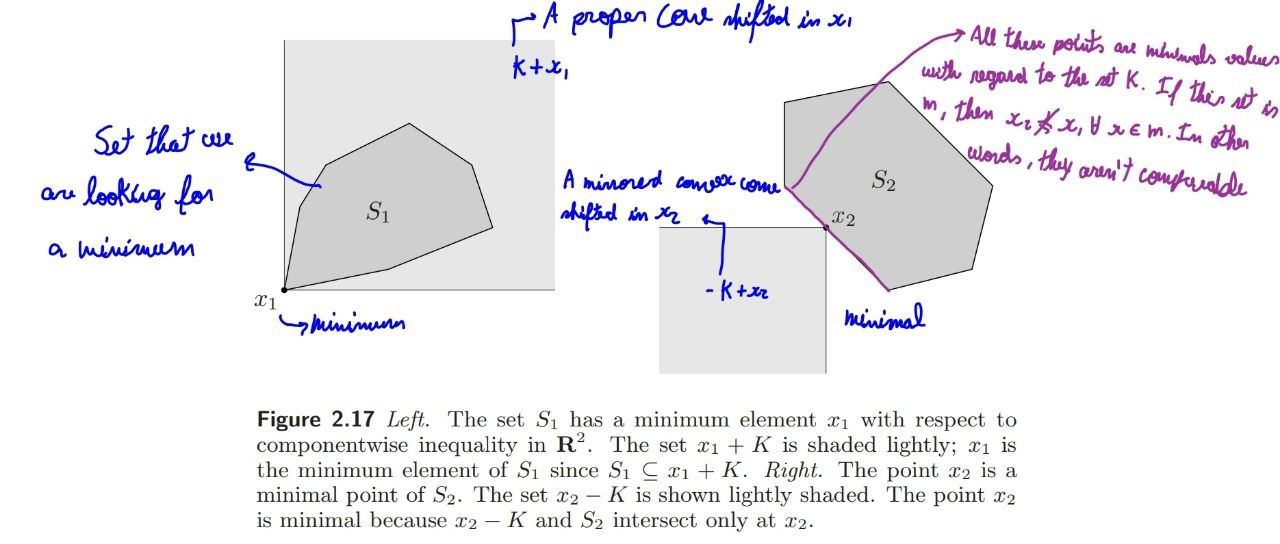
\includegraphics[scale=.5]{figs/minimum_maximum.jpg}
\end{figure}

\subsection{Operations on set and their implications regarding curvature}
\begin{xltabular}[l]{0.5\linewidth}{|X|X|}
    \hline
    \multicolumn{1}{|c|}{Operation} & \multicolumn{1}{|c|}{Curvature}\\
    \hline
    Union \(C = A \cup B \)
    \begin{itemize}[leftmargin=*]
        \item \(C = \left\{ \mathbf{x}\in \mathbb{R}^{n} \mid \mathbf{x} \in A \text{ or } \mathbf{x} \in B \right\}\).
    \end{itemize} & It is neither convex nor concave in most of the cases, even if \(A\) and \(B\) are convex\\
    \hline
    Intersection: $C = A \cap B $
    \begin{itemize}[leftmargin=*]
        \item \(C = \left\{ \mathbf{x}\in \mathbb{R}^{n} \mid \mathbf{x} \in A, \mathbf{x} \in B \right\}\).
    \end{itemize} & It is convex as long as \(A\) and \(B\) are convexes\\
    \hline
    Minkowski sum: $C = A + B $
    \begin{itemize}[leftmargin=*]
        \item \(C = \left\{ \mathbf{x}+\mathbf{y} \in \mathbb{R}^{n} \mid \mathbf{x} \in A, \mathbf{y} \in B \right\}\).
    \end{itemize} & It is convex as long as \(A\) and \(B\) are convexes\\
    \hline
    Minkowski difference: $C = A - B $
    \begin{itemize}[leftmargin=*]
        \item \(C = \left\{ \mathbf{x}-\mathbf{y} \in \mathbb{R}^{n} \mid \mathbf{x} \in A, \mathbf{y} \in B \right\}\).
    \end{itemize} & It is neither convex nor concave in most of the cases, even if \(A\) and \(B\) are convex\\
    \hline
    Offset: $C = A + k $
    \begin{itemize}[leftmargin=*]
        \item \(C = \left\{ \mathbf{x}+k \in \mathbb{R}^{n} \mid \mathbf{x} \in A, k \in \mathbb{R} \right\}\).
    \end{itemize} & It is convex as long as \(A\) and \(B\) are convexes\\
    \hline
    Set scaling: $C = \alpha A$
    \begin{itemize}[leftmargin=*]
        \item \(C = \left\{ \alpha \mathbf{x} \mid \mathbf{x} \in A \right\}\).
    \end{itemize} & It is convex as long as \(A\) and \(B\) are convexes\\
    \hline
    Cartesian product: $C = A \times B $
    \begin{itemize}[leftmargin=*]
        \item \(C = \left\{ (\mathbf{x}, \mathbf{y}) \mid \mathbf{x} \in A, \mathbf{y} \in \mathbb{B} \right\}\).
    \end{itemize} & It is convex as long as \(A\) and \(B\) are convexes\\
    \hline
\end{xltabular}

\subsection{Analitical strategies to prove that a set is convex}
\subsubsection{Get a middle point between extremes of the set and see whether it leads to a contradiction (useful to prove nonconvexity)}
The set \(S \in \mathbb{R}^{n}\) is convex iff it contains all convex combinations of the points belonging to \(S\), i.e.,
\begin{align}
    \mathbf{w} = \theta \mathbf{x} + (1-\theta)\mathbf{y} \in S \;\forall\; \mathbf{x}, \mathbf{y} \in S, 0\leq\theta\leq 1
\end{align}
\begin{itemize}
    \item Note that \(\mathbf{w}\) is a point between \(\mathbf{x}\) and \(\mathbf{y}\), i.e., \(\mathbf{x} \preceq_K \mathbf{w} \preceq_k \mathbf{y}\), where \(K\) is a given cone set.
    \item For instance, if \(S = \left\{ \mathbf{v} \in \mathbb{R}_{+}^{2} \mid v_0v_1 \leq 1 \right\}\), we can show its nonconvexity with the following steps:
    \begin{enumerate}
        \item Take extreme points that belong to this set. In this example, consider the case where \(x_1 \gg 0\) and \(y_0 \gg 0\)
        \item Apply the consequence of this extreme case on other vector elements. In this example, it leads to \(x_0 \rightarrow 0\) and \(y_1 \rightarrow 0\).
        \item Set \(\mathbf{w}\) to the middle point between \(\mathbf{x}\) and \(\mathbf{y}\), i.e., \(\theta = 0.5\).
        \item Try to find conditions, on element-by-element of \(\mathbf{w}\), that lead to a contradiction of the initial condition. In this example, the equation \(w_1 = \theta x_1 + (1-\theta)y_1\) makes us conclude that \(w_0 \rightarrow 0\), regarding that \(\mathbf{w} \in S\). On the other hand, the equation \(w_0 = \theta x_0 + (1-\theta)y_0\) makes us to conclude that \(w_0 \gg 0\), regarding that \(\mathbf{w} \in S\).
        \item The contradiction leads us to prove that \(\mathbf{w} \not\in S\)
    \end{enumerate}
\end{itemize}
\begin{figure}[H]
    \centering
    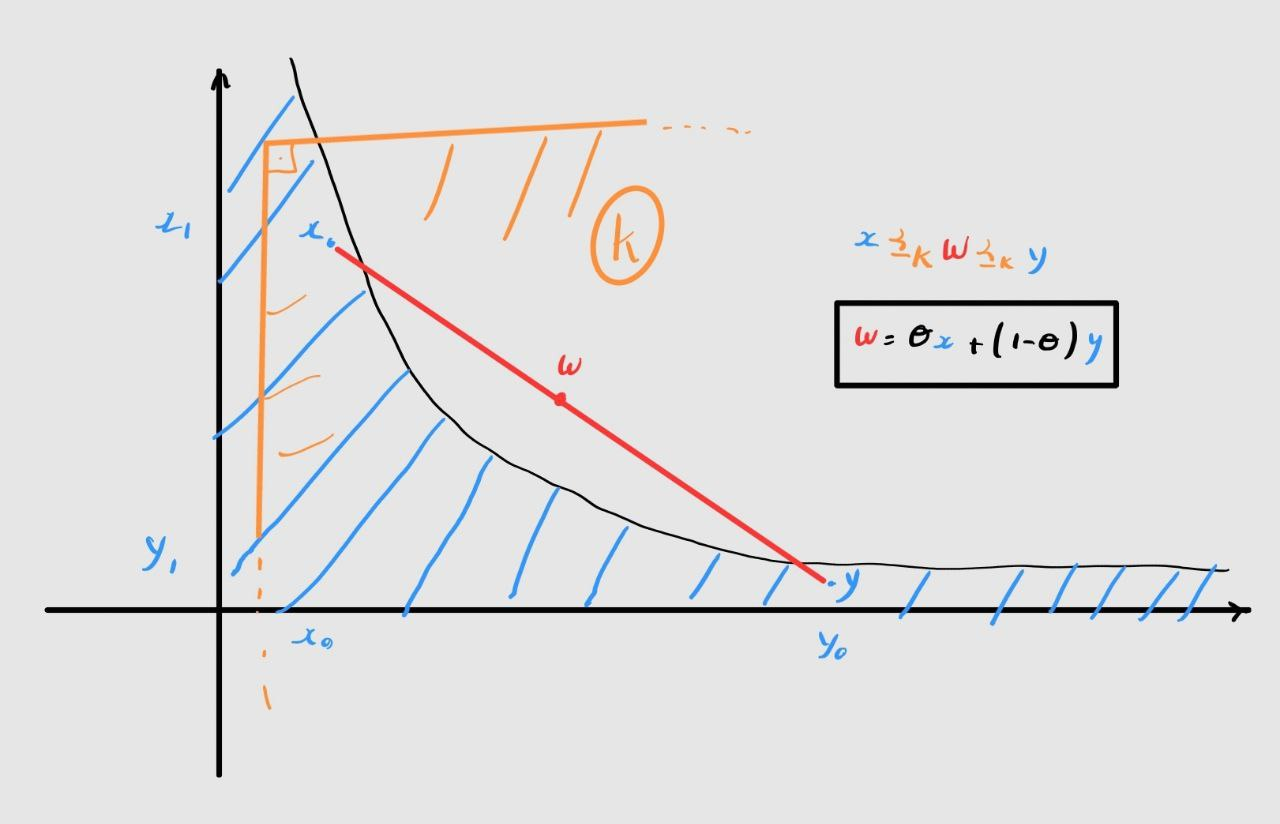
\includegraphics[scale = 0.2]{figs/2.8_set.png}
\end{figure}

\subsubsection{Apply the convex combination and verify whether it holds for all possible combinations}

The set \(S \in \mathbb{R}^{n}\) is convex iff it contains all convex combinations of the points belonging to \(S\), i.e.,
\begin{align}
    \mathbf{w} = \theta \mathbf{x} + (1-\theta)\mathbf{y} \in S \;\forall\; \mathbf{x}, \mathbf{y} \in S, 0\leq\theta\leq 1
\end{align}
\begin{itemize}
    \item Note that \(\mathbf{w}\) is a point between \(\mathbf{x}\) and \(\mathbf{y}\), i.e., \(\mathbf{x} \preceq_K \mathbf{w} \preceq_k \mathbf{y}\), where \(K\) is a given cone set.
    \item For instance, if \(S = \left\{ \mathbf{v} \in \mathbb{R}_{++}^{2} \mid v_0/v_1 \leq 1 \right\}\), we can show its convexity with the following steps:
    \begin{itemize}
        \item Apply the property of the set on the convex combination regarding \(\mathbf{x}\) and \(\mathbf{y}\), which are known to belong to \(S\). Thus, \(\mathbf{w} = \mathbf{x} + (1-\theta)\mathbf{y} = (\theta x_0 + (1 - \theta)y_0, \theta x_1 + (1 - \theta)y_1)\)
        \item Assume that the resulting point of the convex combination, \(\mathbf{w}\), which is between \(\mathbf{x}\) and \(\mathbf{y}\), also belongs to \(S\), and apply the conditional that makes any point belong to \(S\). That is, \(\frac{\theta x_0 + (1 - \theta)y_0}{\theta x_1 + (1 - \theta)y_1} \geq 1\).
        \item Manipulate the expression in a way that you see that this inequation hold for any \(\mathbf{x}, \mathbf{y} \in S\) (or discover that is does not hold). It is usually useful to apply the conditions from the fact that \(\mathbf{x}, \mathbf{y} \in S\) to infer whether the equation/inequation holds. In this example, \(\frac{x_0}{x_1}\frac{\theta}{y_1} + \frac{y_0}{y_1} \frac{1 - \theta}{x_1} \geq \frac{\theta}{y_1} + \frac{1 - \theta}{x_1}\) is clearly true for any \(\mathbf{x}, \mathbf{y} \in S\). Then, \(\mathbf{w} \in S\).
    \end{itemize}
\end{itemize}

\section{Fuctions}
\subsection{Categories of functions regarding its curvature for CVX}
\begin{itemize}
    \item On CVX, for functions with multiple arguments (a vector as input), the curvature categories are always considered jointly \autocite{DCPRulesetCVX}.
	\item The CVX optimization package, and, apparently, its derivatives (CVXPY, Convex.jl, CVXR...) categorize the functions as follows \autocite{DCPRulesetCVX}:
\end{itemize}
\subsubsection{Convex}
\begin{align}
    f(\theta\mathbf{x}+(1-\theta)\mathbf{y}) \leq \theta f(\mathbf{x}) + (1-\theta)f(\mathbf{y}),\;\forall\; \mathbf{x}, \mathbf{y} \in \dom{f}, 0\leq\theta\leq 1
    \label{eq:convex-rule}
\end{align}
\begin{itemize}
    \item \(f: \dom{f} \rightarrow \mathbb{R}\), where \(\dom{f} \subseteq \mathbb{R}^{n}\).
    \item The Eq.\eqref{eq:convex-rule} implies that \(\dom{f}\) is a convex set, that is, all points for any line segment within \(\dom{f}\) belong to it.
    \item The Eq.\eqref{eq:convex-rule} implies that any line segment within \(\dom{f}\) gives a convex graph (bowl-shaped).
    \item Graphically, any line segment between \((\mathbf{x}, f(\mathbf{x}))\) and \((\mathbf{y}, f(\mathbf{y}))\) lies always above the graph \(f\). If the line touches the graph but does not cross it, then the function is strictly convex.
    \begin{figure}[H]
        \centering
        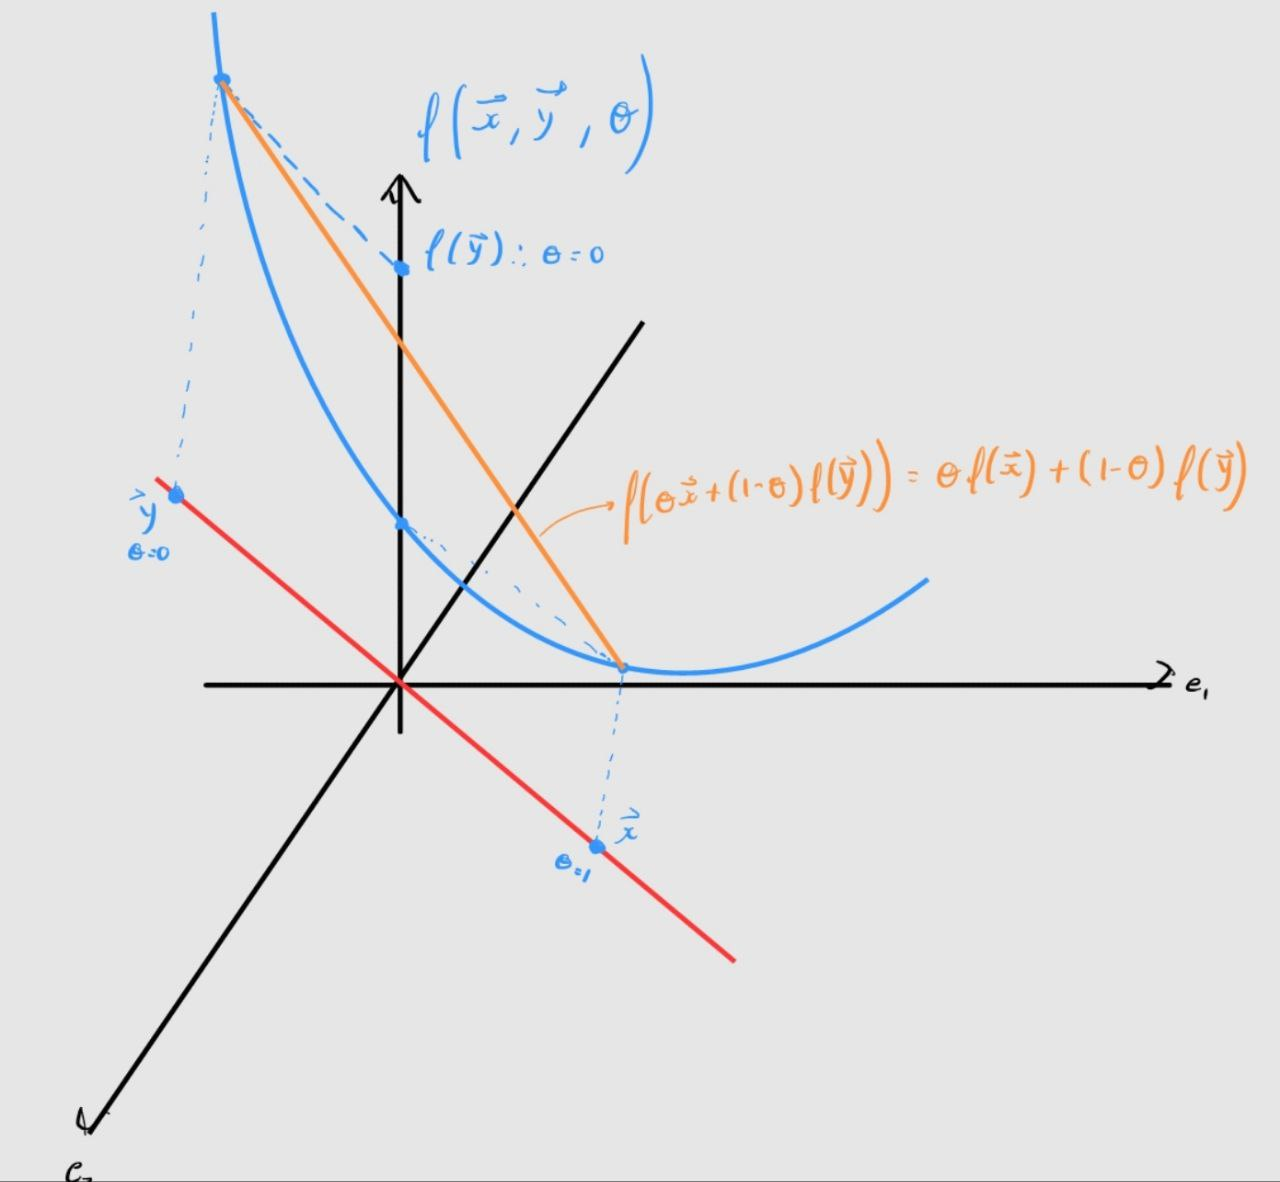
\includegraphics[scale=.2]{figs/convex.png}
    \end{figure}
    \item It is guaranteed that \(\exists!\; \mathbf{x}^{\star} \in \mathbb{R}^{n} \mid f(\mathbf{x}^{\star}) \leq f(\mathbf{y})\;\forall\;\mathbf{y}\in\dom{f}\), and \(\nabla f(\mathbf{y}) = \mathbf{0}\) iff \(\mathbf{y} = \mathbf{x}^{\star}\). This \(\mathbf{x}^{\star}\) is the global minimum.
    \item If \(f\) is (strictly convex) convex, then \(-f\) is (strictly concave) concave.
\end{itemize}
\subsubsection{Concave}
\begin{align}
    f(\theta\mathbf{x}+(1-\theta)\mathbf{y}) \geq \theta f(\mathbf{x}) + (1-\theta)f(\mathbf{y}),\;\forall\; \mathbf{x}, \mathbf{y} \in \dom{f}, 0\leq\theta\leq 1
    \label{eq:concave-rule}
\end{align}
\begin{itemize}
    \item \(f: \dom{f} \rightarrow \mathbb{R}\), where \(\dom{f} \subseteq \mathbb{R}^{n}\).
    \item The Eq.\eqref{eq:concave-rule} implies that \(\dom{f}\) is a convex set, that is, all points for any line segment within \(\dom{f}\) belong to it.
    \item The Eq.\eqref{eq:concave-rule} implies that any line segment within \(\dom{f}\) gives a concave graph (hyperhyperbola-shaped).
    \item Graphically, any line segment between \((\mathbf{x}, f(\mathbf{x}))\) and \((\mathbf{y}, f(\mathbf{y}))\) lies always below the graph \(f\). If the line touches the graph but does not cross it, then the function is strictly concave.
    \begin{figure}[H]
        \centering
        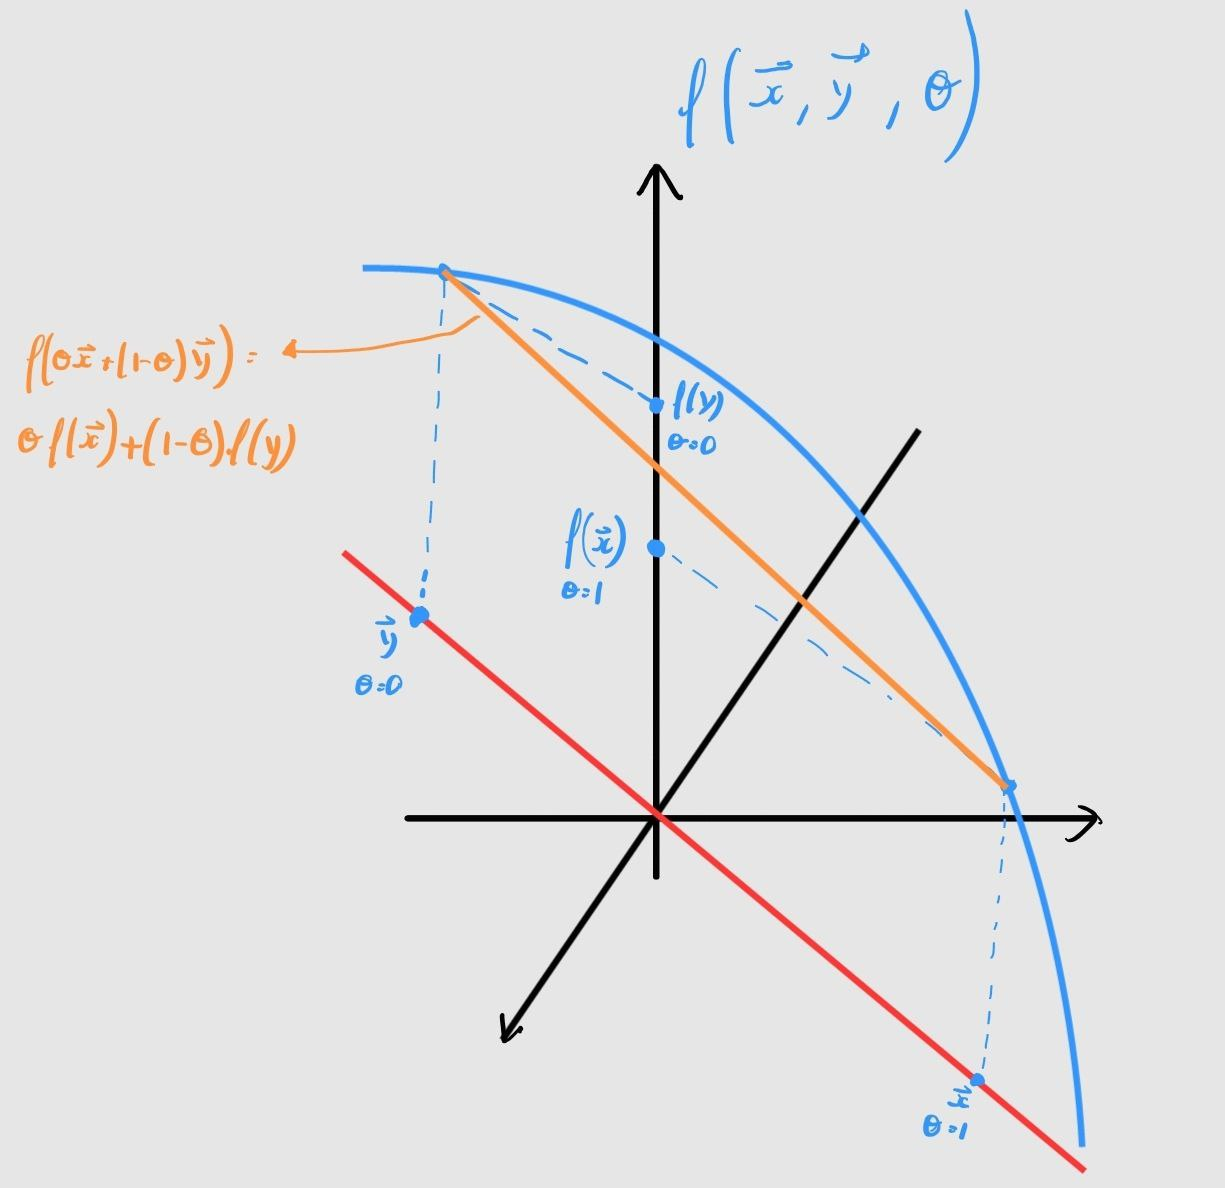
\includegraphics[scale=.2]{figs/concave.png}
    \end{figure}
    \item It is guaranteed that \(\exists!\; \mathbf{x}^{\star} \in \mathbb{R}^{n} \mid f(\mathbf{x}^{\star}) \leq f(\mathbf{y})\;\forall\;\mathbf{y}\in\dom{f}\), and \(\nabla f(\mathbf{y}) = \mathbf{0}\) iff \(\mathbf{y} = \mathbf{x}^{\star}\). This \(\mathbf{x}^{\star}\) is the global maximum. 
    \item If \(f\) is (strictly concave) concave, then \(-f\) is (strictly convex) convex.
\end{itemize}
\subsubsection{Affine}
\begin{align}
    f(\theta \mathbf{x} + (1-\theta)\mathbf{y}) = \theta f(\mathbf{x}) + (1-\theta)f(\mathbf{y}),\;\forall\; \mathbf{x}, \mathbf{y} \in \mathbb{R}^{n}, \theta\in\mathbb{R}
\end{align}
\begin{itemize}
    \item \(f: \mathbb{R}^{n} \rightarrow \mathbb{R} \therefore \dom{f} = \mathbb{R}^{n}\).
    \item \(\dom{f}\) must be infinite since \(\theta\) is not restricted to an interval.
    \item The affine function has the following characteristic
    \begin{figure}[H]
        \centering
        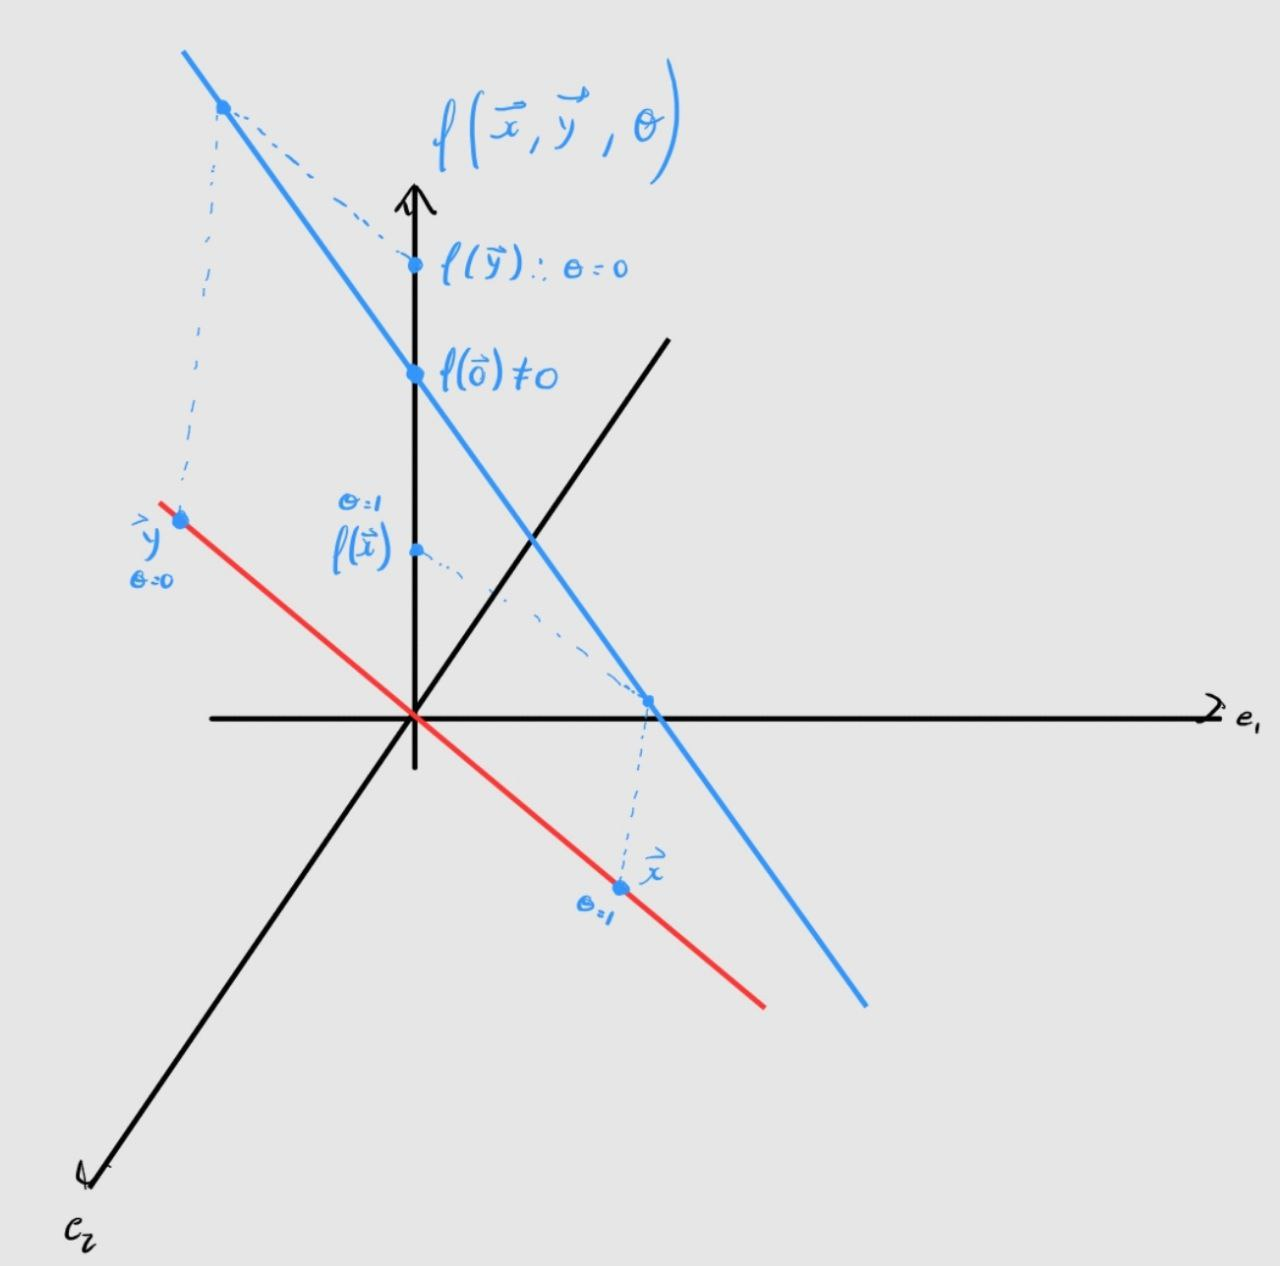
\includegraphics[scale=.2]{figs/affine.png}
    \end{figure}
    \item For all \(\mathbf{x}, \mathbf{y} \in \mathbb{R}^{n}\), \(f\) yields a line with the variation of \(\theta\).
    \item The affine function is a broader category that encompasses the class of linear functions. The main difference is that linear functions must have its origin fixed after the transformation, whereas affine functions do not necessarily have it (when not, this makes the affine function nonlinear). Mathematically, the linear function shall obey the following relation
    \begin{align}
        f(\alpha \mathbf{x} + \beta \mathbf{y}) = \alpha f(\mathbf{x}) + \beta f(\mathbf{y}),\;\forall\; \mathbf{x}, \mathbf{y} \in \mathbb{R}^{n}, \alpha,\beta\in\mathbb{R}.
    \end{align}
    When \(\alpha=\beta=0\), \(f(\mathbf{0}) = 0\). It leads to the following graph
    \begin{figure}[H]
        \centering
        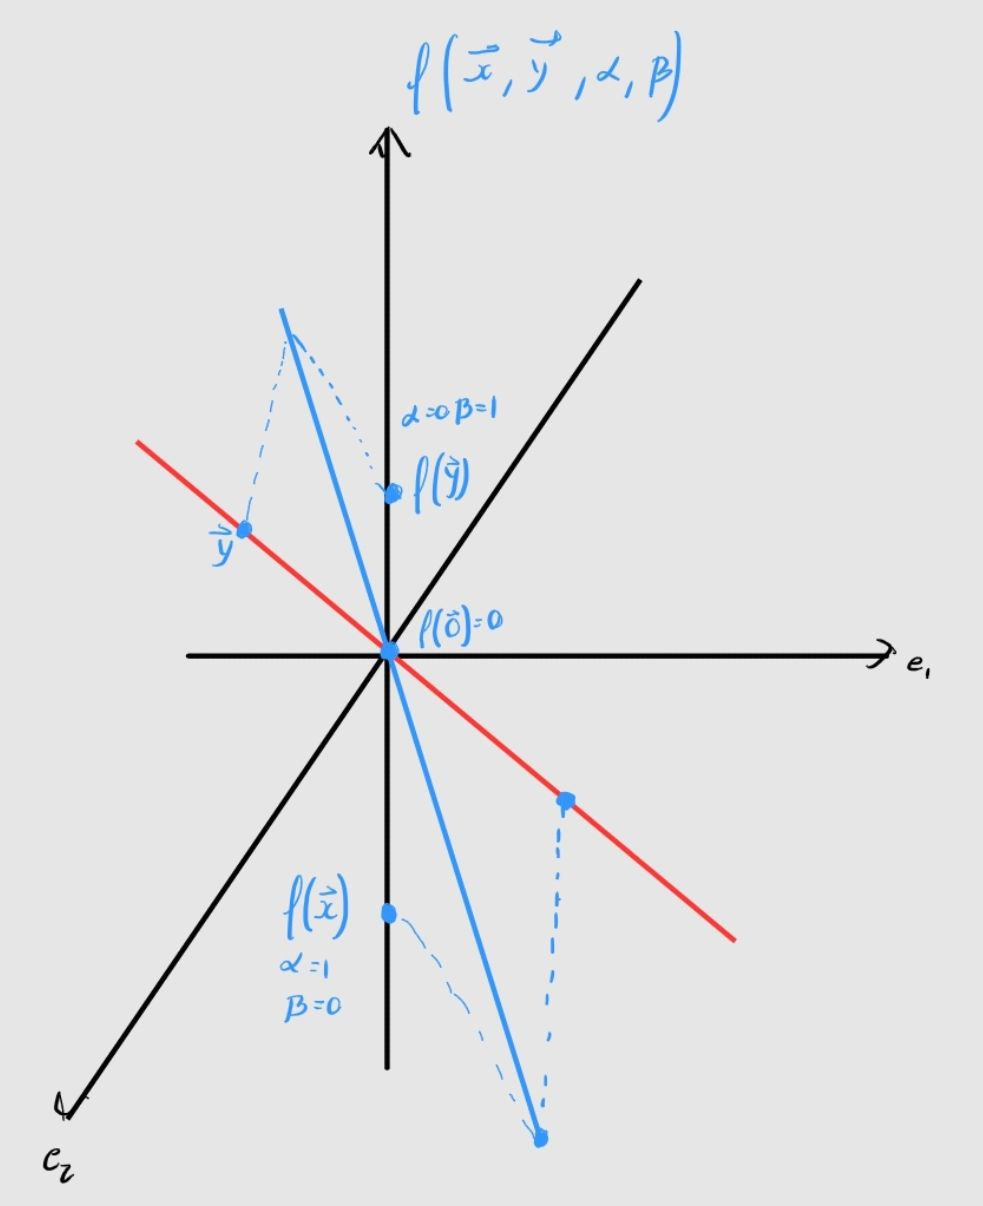
\includegraphics[scale=.2]{figs/linear.png}
    \end{figure}
    \item We can think of an affine function as a linear transformation plus a shift from the origin.
    \item Affine functions are both convex and concave.
\end{itemize}
\subsubsection{Constant}
\begin{align}
    f(\theta \mathbf{x} + (1-\theta)\mathbf{y}) = k,\;\forall\; \mathbf{x}, \mathbf{y} \in \dom{f}, \theta \in \mathbb{R}
\end{align}
\begin{itemize}
    \item \(f: \mathbb{R}^{n} \rightarrow \mathbb{R} \therefore \dom{f} = \mathbb{R}^{n}\).
    \item \(\dom{f}\) must be infinite since \(\theta\) is not restricted to an interval.
    \item \(k\in \mathbb{R}\) is a constant.
    \item It is a special case of affine function.
    \item A constant function is convex and concave, simultaneously.
\end{itemize}
\subsubsection{Unkown}
\begin{itemize}
    \item Nonconvex and nonconcave functions do not satisfy the convexity or concavity rule and are categorized as unknown curvature.
    \item Possibly, convex and/or concave functions can also be categorized as unknown if it does not follow the DCP ruleset.
\end{itemize}
\subsection{Categories of functions regarding its optimization variables}
\begin{xltabular}[l]{\linewidth}{|>{\hsize=.25\hsize}X|>{\hsize=.25\hsize}X|}
    % \caption{Caption.\label{tab:xltabular}}\\[\belowcaptionskip]
    \hline
    \(\mathbf{x}\in \mathbb{R}^{n}\)     & Continuous optimization     \\ \hline
    \(\mathbf{x}\in \mathbb{Z}^{n}\)     & Integer optimization        \\ \hline
    \(x_1,x_2,\dots,x_k \in \mathbb{R}\) and \(x_{k+1}, \dots, x_n \in \mathbb{Z}\)         & Mixed-optimization        \\ \hline
\end{xltabular}

\subsection{Table of known functions}
\begin{xltabular}{\textwidth}{|>{\setlength\hsize{1\hsize}\setlength\linewidth{\hsize}}X|>{\setlength\hsize{.9\hsize}\setlength\linewidth{\hsize}}X|>{\setlength\hsize{1.1\hsize}\setlength\linewidth{\hsize}}X|}%{| >{\hsize=.5\hsize}X | >{\hsize=1.5\hsize}X |}
    \hline
    \multicolumn{3}{|c|}{Functions and their implications regarding curvatuve} \\
    \hline
    \multicolumn{1}{|c|}{Function} & \multicolumn{1}{|c|}{Curvature and monoticity} & \multicolumn{1}{|c|}{Comments} \\
    \hline
    Matrix functions \(f: \mathbb{R}^n \rightarrow \mathbb{R}^m\)
    \begin{itemize}[leftmargin=*]
        \item $f(\mathbf{x}) = \mathbf{Ax} + \mathbf{b}$, where \(\mathbf{A} \in \mathbb{R}^{m\times n}, \mathbf{b} \in \mathbb{R}^{m}, \mathbf{x} \in \mathbb{R}^{n}\)
    \end{itemize} & \vspace{-3.5ex} \begin{itemize}[leftmargin=*]
	\item Affine.
	\item If \(\mathbf{b} = \mathbf{0}\), then \(f(\mathbf{x}) = \mathbf{Ax}\) is a linear function.
\end{itemize} & \vspace{-3.5ex} \begin{itemize}[leftmargin=*]
        \item A special case of the linear function is when \(\mathbf{A} = \mathbf{c}^\mathsf{T}\). In this case, we have \(f(\mathbf{x}) = \mathbf{c}^\mathsf{T}\mathbf{x}\), which is the inner product between the vector \(\mathbf{c}\) and \(\mathbf{x}\).
        \item The inverse image of \(C\), \(f^{-1}(C) = \left\{ \mathbf{x} \mid f(\mathbf{x}) \in C \right\}\), is also convex.
        \item The \emph{linear matrix inequality} (LMI), \(\mathbf{A}(\mathbf{x}) = x_1\mathbf{A}_1 + \dots + x_n\mathbf{A}_n \preceq \mathbf{B}\), is a special case of sums of matrix functions. In other words, \(f(S) = \left\{ \mathbf{x} \mid \mathbf{A}(\mathbf{x}) \preceq \mathbf{B} \right\}\) is a convex set if \(S\) is convex. Many optimization problems can be formulated as LMI problems and solved optimally.
    \end{itemize} \\
    \hline
    Exponential function \(f: \mathbb{R} \rightarrow \mathbb{R}\)
    \begin{itemize}[leftmargin=*]
        \item \(f(x)=e^{ax} \in \mathbb{R}\), where \(a \in \mathbb{R}\)
    \end{itemize} & Convex. & \\
    \hline
    Quadratic function \(f: \mathbb{R}^{n} \rightarrow \mathbb{R}\)
    \begin{itemize}[leftmargin=*]
        \item \(f(\mathbf{x}) = a \mathbf{x}^\mathsf{T}\mathbf{P} \mathbf{x} + \mathbf{p}^\mathsf{T} \mathbf{x} + r \in \mathbb{R}\), where \(\mathbf{x},\mathbf{p} \in \mathbb{R}^{n}, \mathbf{P} \in \mathbb{R}^{n\times n}\), and \(a,b \in \mathbb{R}\)
    \end{itemize} & It depends on the matrix \(\mathbf{P}\): \begin{itemize}[leftmargin=*]
        \item \(f\) is convex iff \(\mathbf{P} \succeq \mathbf{0}\).
        \item \(f\) is strictly convex iff \(\mathbf{P} \succ \mathbf{0}\).
        \item \(f\) is concave iff \(\mathbf{P} \preceq \mathbf{0}\).
        \item \(f\) is strictly concave iff \(\mathbf{P} \prec \mathbf{0}\).
    \end{itemize} & \\
    \hline
    Quadratic-over-linear function \(f: \mathbb{R}^{n} \times \mathbb{R}_{++}\)
    \begin{itemize}[leftmargin=*]
    \item \(f(\mathbf{x}, y) = \norm{\mathbf{x}}^2/y\), where \(\mathbf{x} \in \mathbb{R}^{n}\) and \(y \in \mathbb{R}_{++}\)
    \end{itemize} & Convex & \vspace{-3.5ex} 
    \begin{itemize}[leftmargin=*]
        \item It appeared for the first time in Stephen Boyd's Book \autocite{boydConvexOptimization2004} with \(n=1\), but then it appeared generalized for \(n\)-dimensional vector on the exercises \autocite{boydAdditionalExercisesConvex}.
    \end{itemize}
    \\
    \hline
    Power function \(f: \mathbb{R}_{++} \rightarrow \mathbb{R} \) \begin{itemize}[leftmargin=*]
        \item \(f(x) = x^{a}\)
    \end{itemize} & It depends on \(a\) \begin{itemize}[leftmargin=*]
        \item \(f\) is convex iff \(a\geq 1\) or \(a\leq 0\).
        \item \(f\) is concave iff \(0\leq a \leq 1\).
    \end{itemize} & \vspace{-3.5ex}
    \begin{itemize}[leftmargin=*]
        \item Note that it is guaranteed to be convex or concave iff the base power is solely \(x\). For instance, \((x+1)^2\) is convex, but \((x-1)^2\) is nonconvex and nonconcave.
    \end{itemize}\\
    \hline
    Power of absolute value: \(f: \mathbb{R} \rightarrow \mathbb{R}\) \begin{itemize}[leftmargin=*]
        \item \(f(x) = \abs{x}^p\), where \(p\leq 1\).
    \end{itemize} & Convex. & \\
    \hline
    Minkowski distance, \(p\)-norm function, or \(l_p\) norm function: \(f: \mathbb{R}^{n} \rightarrow \mathbb{R}\)
    \begin{itemize}[leftmargin=*]
        \item \(f(\mathbf{x}) = \norm{\mathbf{x}}_{p}\), where \(p \in \mathbb{N}_{++}\).
    \end{itemize} & Convex. & \vspace{-3.5ex} \begin{itemize}[leftmargin=*]
        \item It can be proved by triangular inequality.
    \end{itemize} \\
    \hline
    Maximum element: \(f: \mathbb{R}^{n} \rightarrow \mathbb{R}\)
    \begin{itemize}[leftmargin=*]
        \item \(f(\mathbf{x}) = \max\left\{ x_1, \dots, x_n \right\}\).
    \end{itemize} & Convex. & \\
    \hline
    Minimum element: \(f: \mathbb{R}^{n} \rightarrow \mathbb{R}\)
    \begin{itemize}[leftmargin=*]
        \item \(f(\mathbf{x}) = \min\left\{ x_1, \dots, x_n \right\}\).
    \end{itemize} & Nonconvex and nonconcave in most of the cases. & \\
    \hline
    Maximum function (pointwise maximum): \(f: \mathbb{R}^{n} \rightarrow \mathbb{R}\)
    \begin{itemize}[leftmargin=*]
        \item \(f(\mathbf{x}) = \max\left\{ f_1(\mathbf{x}), \dots, f_n(\mathbf{x}) \right\}\).
    \end{itemize} & \(f\) is convex (concave) if \(f_1, \dots, f_n\) are convex (concave) functions. &
    \vspace{-3.5ex} \begin{itemize}[leftmargin=*]
        \item Its domain \(\dom{f} = \bigcap\limits_{i=1}^{n} \dom{f_i}\) is also convex.
    \end{itemize} \\
    \hline
    Minimum function (pointwise minimum): \(f: \mathbb{R}^{n} \rightarrow \mathbb{R}\)
    \begin{itemize}[leftmargin=*]
        \item \(f(\mathbf{x}) = \min\left\{ f_1(\mathbf{x}), \dots, f_n(\mathbf{x}) \right\}\).
    \end{itemize} & Nonconvex and nonconcave in most of the cases. & \\
    \hline
    Pointwise infimum:
    \begin{itemize}[leftmargin=*]
        \item \(f(\mathbf{x}) = \underset{\mathbf{y} \in \mathcal{A}}{\textnormal{inf }} g(\mathbf{x},\mathbf{y})\).
    \end{itemize} & \(f\) is concave if \(g\) is concave for each \(\mathbf{y}\in \mathcal{A}\). &
    \vspace{-3.5ex} \begin{itemize}[leftmargin=*]
        \item For each value of \(x\), we have an infinite set of points \(\eval{g(x,y)}{y\in \mathcal{A}}\). The value \(f(x)\) will be the greatest value in the codomain of \(f\) that is less than or equal this set.
        \item \(\dom{f} = \left\{ x \mid (x,y) \in \dom{g} \;\forall\; y \in \mathcal{A}, \underset{y \in \mathcal{A}}{\textnormal{ inf }}g(x,y)> -\infty \right\}\).
    \end{itemize} \\
    \hline
    Pointwise supremum:
    \begin{itemize}[leftmargin=*]
        \item \(f(\mathbf{x}) = \underset{\mathbf{y} \in \mathcal{A}}{\textnormal{sup }} g(\mathbf{x},\mathbf{y})\).
    \end{itemize} & \(f\) is convex if \(g\) is convex for each \(\mathbf{y}\in \mathcal{A}\). &
    \vspace{-3.5ex} \begin{itemize}[leftmargin=*]
        \item For each value of \(x\), we have an infinite set of points \(\eval{g(x,y)}{y\in \mathcal{A}}\). The value \(f(x)\) will be the least value in the codomain of \(f\) that is greater than or equal this set.
        \item \(\dom{f} = \left\{ x \mid (x,y) \in \dom{g} \;\forall\; y \in \mathcal{A}, \underset{y \in \mathcal{A}}{\textnormal{ sup }}g(x,y)<\infty \right\}\).
        \item In terms of epigraphs, the pointwise supremum of the infinite set of functions \(\eval{g(x,y)}{y\in \mathcal{A}}\) corresponds to the intersection of the following epigraphs: \(\textnormal{epi } f = \intersection_{y \in \mathcal{A}} \textnormal{epi } g(\cdot, y)\)
    \end{itemize} \\
    \hline
    Logarithm function: \(f: \mathbb{R}_{++} \rightarrow \mathbb{R}\) \begin{itemize}[leftmargin=*]
        \item \(f(x) = \log x\)
    \end{itemize} & Concave and nondecreasing. & \\
    \hline
    Negative entropy function: \(f: \mathbb{R}_{+} \rightarrow \mathbb{R}\)
    \begin{itemize}[leftmargin=*]
        \item \(f(x) = x\log x \)
    \end{itemize} & Convex. & \vspace{-3.5ex}
    \begin{itemize}[leftmargin=*]
        \item When it is defined \(\eval{f(x)}{x=0} = 0 \), \(\dom{f} = \mathbb{R}\).
    \end{itemize} \\
    \hline
    Log-sum-exp function: \(f: \mathbb{R}^{n} \rightarrow \mathbb{R}\)
    \begin{itemize}[leftmargin=*]
        \item \(f(\mathbf{x}) = \log\left( e^{x_1} + \dots+ e^{x_n} \right)\)
    \end{itemize} & Convex. & \vspace{-3.5ex}
    \begin{itemize}[leftmargin=*]
        \item This function is interpreted as the approximation of the maximum element function, since \(\max\left\{ x_1, \dots, x_n \right\} \leq f(\mathbf{x}) \leq \max \left\{ x_1, \dots, x_n \right\} + \log n\)
    \end{itemize} \\
    \hline
    Geometric mean function \(f: \mathbb{R}^{n}\rightarrow \mathbb{R}\)
    \begin{itemize}[leftmargin=*]
        \item \(f(\mathbf{x}) = \left( \Pi_{i=1}^{n} x_i \right)^{1/n}\)
    \end{itemize} & Convex. & \\
    \hline
    Log-determinant function \(f: \mathbb{S}^{n}_{++}\rightarrow \mathbb{R}\)
    \begin{itemize}[leftmargin=*]
        \item \(f(\mathbf{X}) = \log \abs{\mathbf{X}}\)
    \end{itemize} & Convex. & \vspace{-3.5ex}
    \begin{itemize}[leftmargin=*]
        \item \(\mathbf{X}\) is positive semidefinite, i.e., \(\mathbf{X} \succ \mathbf{0} \therefore \mathbf{X}\in \mathbb{S}^{n}_{++}\).
    \end{itemize} \\
    \hline
    Composite function \(f = h\circ g : \mathbb{R}^{n}\rightarrow \mathbb{R}\)
    \begin{itemize}[leftmargin=*]
        \item \(f = g \circ h\), i.e., \(f(\mathbf{x}) = (h\circ g)(\mathbf{x}) = h(g(\mathbf{x}))\), where:
        \begin{itemize}[label=\(\triangleright\)]
            \item \(g: \mathbb{R}^{n}\rightarrow \mathbb{R}^{k}\).
            \item \(h: \mathbb{R}^{k}\rightarrow \mathbb{R}\).
            \item \(\dom{f} = \left\{ \mathbf{x} \in \dom{g}\mid g(\mathbf{x}) \in \dom{h} \right\}\).
        \end{itemize}  %\(\mathbf{x} \in S \subseteq \mathbb{R}^{p}\)
    \end{itemize} & \vspace{-3.5ex}
    \begin{itemize}[leftmargin=*]
        \item Scalar composition: the following statements hold for \(k=1\) and \(n\geq 1\), i.e., \(h: \mathbb{R}\rightarrow \mathbb{R}\) and \(g: \mathbb{R}^{n} \rightarrow \mathbb{R}\):
            \begin{itemize}[label=\(\triangleright\)]
                \item \(f\) is convex if \(h\) is convex, \(\tilde{h}\) is nondecreasing, and \(g\) is convex. In this case, \(\dom{h}\) is either \((-\infty, a]\) or \((-\infty, a)\).
                \item \(f\) is convex if \(h\) is convex, \(\tilde{h}\) is nonincreasing, and \(g\) is concave. In this case, \(\dom{h}\) is either \([a, \infty)\) or \((a, \infty)\).
                \item \(f\) is concave if \(h\) is concave, \(\tilde{h}\) is nondecreasing, and \(g\) is concave.
                \item \(f\) is concave if \(h\) is concave, \(\tilde{h}\) is nonincreasing, and \(g\) is convex.
            \end{itemize}
        \end{itemize}
    \begin{itemize}[leftmargin=*]
        \item Vector composition: the following statements hold for \(k\geq 1\) and \(n\geq 1\), i.e., \(h: \mathbb{R}^{k} \rightarrow \mathbb{R}\) and \(\boldsymbol{g}: \mathbb{R}^{n} \rightarrow \mathbb{R}^{k}\). Hence, \(g(\mathbf{x}) = (g_1 (\mathbf{x}), g_2(\mathbf{x}), \dots, g_k(\mathbf{x}))\) is a vector-valued function (or simply, vector function), where \(g_i: \mathbb{R}^{k} \rightarrow \mathbb{R}\) for \(1 \leq i \leq k\).
        \begin{itemize}[label=\(\triangleright\)]
            \item \(f\) is convex if \(h\) is is convex, \(\tilde{h}\) is nondecreasing in each argument of \(\mathbf{x}\), and \(\left\{ g_i \right\}_{i=1}^{k}\) is a set of convex functions.
            \item \(f\) is convex if \(h\) is is convex, \(\tilde{h}\) is nonincreasing in each argument of \(\mathbf{x}\), and \(\left\{ g_i \right\}_{i=1}^{k}\) is a set of concave functions.
            \item \(f\) is concave if \(h\) is is concave, \(\tilde{h}\) is nondecreasing in each argument of \(\mathbf{x}\), and \(\left\{ g_i \right\}_{i=1}^{k}\) is a set of concave functions.
        \end{itemize}
    \end{itemize}
    Where \(\tilde{h}\) is the extended-value extension of the function \(h\), which assigns the value \(\infty\) (\(-\infty\)) to the point not in \(\dom{h}\) for \(h\) convex (concave).
    & \vspace{-3.5ex}
    \begin{itemize}[leftmargin=*]
    \item The composition function allows us to see a large class of functions as convex (or concave).
    \item For scale composition, the remarkable ones are:
        \begin{itemize}[label=\(\triangleright\)]
            \item If \(g\) is convex then \(f(x) = h(g(\mathbf{x})) = \exp{g(\mathbf{x})}\) is convex.
            \item If \(g\) is concave and \(\dom{g} \subseteq \mathbb{R}_{++}\), then \(f(\mathbf{x}) = h(g(\mathbf{x})) = \log{g(\mathbf{x})}\) is concave.
            \item If \(g\) is concave and \(\dom{g} \subseteq \mathbb{R}_{++}\), then \(f(\mathbf{x}) = h(g(\mathbf{x})) = 1/g(\mathbf{x})\) is convex.
            \item If \(g\) is convex and \(\dom{g} \subseteq \mathbb{R}_{+}\), then \(f(\mathbf{x}) = h(g(\mathbf{x})) = g^{p}(\mathbf{x})\) is convex, where \(p\geq 1\).
            \item If \(g\) is convex then \(f(\mathbf{x}) = h(g(\mathbf{x})) = - \log{\left( -g(x) \right)}\) is convex, where \(\dom{f} = \left\{ \mathbf{x} \mid g(\mathbf{x})<0 \right\}\).
        \end{itemize}
    \item For vector composition, we have the following examples:
        \begin{itemize}[label=\(\triangleright\)]
            \item If \(g\) is an affine function, then \(f = h \circ g\) is convex (concave) if \(h\) is convex (concave).
            \item Let \(h(\mathbf{x}) = x_{\left[ 1 \right]} + \dots + x_{\left[ r \right]}\) be the sum of the \(r\) largest components of \(\mathbf{x} \in \mathbb{R}^{k}\). If \(g_1, g_2, \dots, g_k\) are convex, where \(\dom{g_i} = \mathbb{R}^{n}\), then \(f = h\circ g\), which is the pointwise sum of the largest \(g_i\)'s, is convex.
            \item \(f = h\circ g\) is a convex function when \(h(\mathbf{x}) = \log\left( \sum_{i=1}^{k} e^{x_i} \right)\) and \(g_1, g_2, \dots, g_k\) are convex functions.
            \item For \(0<p \leq 1\), the function \(h(\mathbf{x}) = \left( \sum_{i=1}^{k} x_i^p \right)^{1/p}\), where \(\dom{h} = \mathbb{R}_+^{n}\), is concave. If \(g_1, g_2, \dots, g_k\) are concaves (convexes) and nonnegatives, then \(f = h \circ g\) is concave (convex).
        \end{itemize}
    \end{itemize}\\
    \hline
    Nonnegative weighted sum: \(f: \dom{f} \rightarrow \mathbb{R}\)
    \begin{itemize}
        \item \(f(\mathbf{x}) = \sum_{i=1}^{m} w_if_i(\mathbf{x})\), where \(w\geq 0\).
    \end{itemize} & \vspace{-3.5ex} \begin{itemize}[leftmargin=*]
        \item If \(f_1, f_2, \dots, f_m\) are convex or concave functions, then \(f\) is a convex or concave function, respectively.
        \item If \(f_1, f_2, \dots, f_m\) are strictly convex or concave functions, then \(f\) is a strictly convex or concave function, respectively.
    \end{itemize} & \vspace{-3.5ex} \begin{itemize}[leftmargin=*]
        \item Special cases are when
        \begin{itemize}
            \item \(f = w f\) (a nonnegative scaling)
            \item \(f = f_1 + f_2\) (sum).
        \end{itemize}
    \end{itemize}\\
    \hline
    Addition/subtraction by a constant \(f: \dom{f} \rightarrow \mathbb{R}\)
    \begin{itemize}
        \item \(f(\mathbf{x}) = g(\mathbf{x}) \pm k\), where \(k \in \mathbb{R}\) is a constant and \(g: \mathbb{R}^{n}\rightarrow \mathbb{R}\).
    \end{itemize}&\vspace{-3.5ex} \begin{itemize}[leftmargin=*]
        \item If \(g\) is convex (concave), then \(f\) is convex (concave)
    \end{itemize}&\\
    \hline
    Integral function \(f: \mathbb{R}^{n}\rightarrow \mathbb{R}\):
    \begin{itemize}
        \item \(f(\mathbf{x}) = \int_\mathcal{A} w(\mathbf{y}) g(\mathbf{x},\mathbf{y}) \diff \mathbf{y}\), where \(\mathbf{y} \in \mathcal{A} \subseteq \mathbb{R}^{m}\), and \(w: \mathbb{R}^{m} \rightarrow \mathbb{R}\).
    \end{itemize} & If \(g\) is convex in \(\mathbf{x}\) for each \(\mathbf{y}\in \mathcal{A}\) and if \(w(\mathbf{y}) \geq 0, \;\forall\; \mathbf{y}\in \mathcal{A}\), then \(f\) is convex (provided the integral exists). & \\
    \hline
    \hline
    Perspective function \(f: \mathbb{R}^{n} \times \mathbb{R}_{++} \rightarrow \mathbb{R}^{n}\)
    \begin{itemize}[leftmargin=*]
        \item \(f(\mathbf{x}, t) = \mathbf{x}/t\), where \(\mathbf{x} \in \mathbb{R}^{n}, t \in \mathbb{R}_{++}\), and \((\mathbf{x}, t) \in \dom{f}\).
    \end{itemize}
    & It is a convex function as long as \(\dom{f}\) is also convex & \vspace{-3.5ex} \begin{itemize}[leftmargin=*]
        \item The perspective function decreases the dimension of the function domain since \(\textnormal{dim}(\dom{f}) = n+1\).
        \item Its effect is similar to the pin-hole camera.
        \item If \(S \subseteq \dom{f} \subseteq \mathbb{R}^{n} \times \mathbb{R}_{++}\) is a convex set, then its image, \(f(S) = \left\{ f(\mathbf{x})|\mathbf{x}\in S \right\} \subseteq \mathbb{R}^{n}\), is also convex.
        \item The inverse image is also convex, that is, if \(C \subseteq \mathbb{R}^{n}\) is convex, then \(f^{-1}(C) = \left\{ (\mathbf{x}, t) \in \mathbb{R}^{n+1} \mid \mathbf{x}/t \in C, t>0 \right\}\) is also convex.
    \end{itemize} \\
    \hline
    Projective (or linear-fractional) function, \(f: \mathbb{R}^{n} \rightarrow \mathbb{R}^{m}\)
    \begin{itemize}[leftmargin=*]
        \item \(f = p \circ g\), i.e., \(f(\mathbf{x}) = (p\circ g)(\mathbf{x}) = p(g(\mathbf{x}))\), where
            \begin{itemize}[label={$\triangleright$}]
                \item \(g: \mathbb{R}^{n} \rightarrow \mathbb{R}^{m+1}\) is an affine function given by \(g(\mathbf{x}) = \begin{bmatrix}
                    \mathbf{A}\\
                    \mathbf{c}^\mathsf{T}
                \end{bmatrix} \mathbf{x} + \begin{bmatrix}
                    \mathbf{b} \\
                    d
                \end{bmatrix}\), being \(\mathbf{A}\in \mathbb{R}^{m \times n}, \mathbf{b} \in \mathbb{R}^{m}, \mathbf{c} \in \mathbb{R}^{n}\), and \(d \in \mathbb{R}\).
                \item \(p: \mathbb{R}^{m+1} \rightarrow \mathbb{R}^{m}\) is the perspective function.
            \end{itemize}
        \item \(f(\mathbf{x}) = \mathcal{P}^{-1}(\mathbf{Q}\mathcal{P}(\mathbf{x}))\)
            \begin{itemize}[label={$\triangleright$}]
                \item \(\mathcal{P}(\mathbf{x}) = \left\{ (t\mathbf{x}, t) \mid t \geq 0 \right\} \subset \mathbb{R}^{n+1}\)
                \item \(\mathbf{Q} = \begin{bmatrix}
                    \mathbf{A} & \mathbf{b} \\
                    \mathbf{c}^\mathsf{T} & d
                \end{bmatrix} \in \mathbb{R}^{(m+1)\times(n+1)}\)
            \end{itemize}
    \end{itemize} & Yes, if \(S \subseteq \dom{f}\) is a convex set, then its image, \(f(S) = \left\{ f(\mathbf{x})|\mathbf{x}\in S \right\} \subseteq \mathbb{R}^{n}\), is also convex. & \vspace{-3.5ex} \begin{itemize}[leftmargin=*]
        \item The linear and affine functions are special cases of the linear-fractional function.
        \item \(\dom{f} = \left\{ \mathbf{x} \in \mathbb{R}^{n} \mid \mathbf{c}^\mathsf{T} \mathbf{x} + d > 0 \right\}\)
        \item \(\mathcal{P}(\mathbf{x}) \subset \mathbb{R}^{n+1}\) is a ray set that begins at the origin and its last component takes only positive values. For each \(\mathbf{x} \in \dom{f}\), it is associated a ray set in \(\mathbb{R}^{n+1}\) in this form. This (projective) correspondence between all points in \(\dom{f}\) and their respective sets \(\mathcal{P}\) is a biunivocal mapping.
        \item The linear transformation \(\mathbf{Q}\) acts on these rays, forming another set of rays.
        \item Finally we take the inverse projective transformation to recover \(f(\mathbf{x})\).
    \end{itemize}\\
    \hline
\end{xltabular}

\section{General approaches to convexity analysis}
\begin{itemize}
    \item Assume that the objective function of convex and proceed.
    \begin{itemize}
        \item It may lead to errors.
    \end{itemize}
    \item Verify analytically whether the problem is convex or not (vide Sec. \ref{sec:analytical-convex}).
    \begin{itemize}
        \item The basic approach is the first- and second-order conditions.
        \item It usually leads to complicated analysis.
    \end{itemize}
    \item Construct the problem as convex from the DCP ruleset and a ``atom library'', which is a set of basic functions that preserve convexity/concavity (vide Sec. \ref{cvx-dcp}).
    \begin{itemize}
        \item It is restricted to the atom library and DCP ruleset, but the convexity verification is automatic.
        \item It usually involves adding auxiliary variables and reformulating the original optimization problem in order to get an expression that obeys the CDP ruleset \autocite{HomeConvexJl}.
        \item The manipulation of the original problem by using operations that preserve the convexity/concavity is called convex calculus\autocite{boydDisciplinedConvexProgramming}.
        \item The reformulation usually leads to a new optimization problem that is not equal to the original one. However, they are equivalents, that is, if your find the solve the reformulated problem, then you also find the solution to the original problem.
    \end{itemize}
\end{itemize}

\section{Analytical strategies to prove that a function is convex}
\label{sec:analytical-convex}
\subsection{First-order condition of convexity (apparently too complicated to prove it)}
\begin{align}
    f(\mathbf{y}) \geq f(\mathbf{x}) + \nabla f (\mathbf{x})^\mathsf{T} (\mathbf{y} - \mathbf{x}),\forall\;\mathbf{x},\mathbf{y} \in \dom{f}, \mathbf{x}\neq\mathbf{y}
\end{align}
\begin{itemize}
    \item \(\nabla f (\mathbf{x})\): gradient vector.
    \item This inequation says that the first-order Taylor approximation is a \emph{underestimator} for convex functions.
    \item The first-order condition requires that \(f\) is differentiable.
\end{itemize}
\subsection{Second-order condition of convexity}
\begin{align}
    \mathbf{H}\succeq \mathbf{0}
\end{align}
\begin{itemize}
    \item In other words, the Hessian matrix \(\mathbf{H}\) is a positive semidefinite matrix.
    \item The graphic of the curvature has a positive (upward) curvature at \(\mathbf{x}\).
    \item If \(\mathbf{H}\succ\mathbf{0}, \forall\; \mathbf{x} \in \dom{f}\), then \(f\) is strictly convex. But if \(f\) is strictly convex, not necessarily \(\mathbf{H}\succ\mathbf{0},\forall\; \mathbf{x} \in \dom{f}\). Therefore, strict convexity can only be partially characterized.
\end{itemize}
\subsection{Convexity definition}
\begin{align}
    f(\theta\mathbf{x}+(1-\theta)\mathbf{y}) \leq \theta f(\mathbf{x}) + (1-\theta)f(\mathbf{y}),\;\forall\; \mathbf{x}, \mathbf{y} \in \dom{f}, 0\leq\theta\leq 1
\end{align}
\begin{itemize}
	\item If \(f\) is continuous, it is enough (and usually convenient as well) to check if
    \begin{align}
        f\left( \dfrac{\mathbf{x}+\mathbf{y}}{2} \right) \leq \dfrac{f(\mathbf{x}) + f(\mathbf{y})}{2}
    \end{align}
\end{itemize}

\section{CVX and Disciplined Convex Programming (DCP)}
\label{cvx-dcp}
\subsection{Introduction}
\begin{itemize}
    \item CVX is a Matlab package for constructing and solving Disciplined Convex Programs (DCP's).
    \item Disciplined convex programming is a methodology for constructing convex optimization problems proposed by Michael Grant, Stephen Boyd, and Yinyu Ye.
    \item The CVX package is also implemented in other programming languages:
    \begin{itemize}
        \item Julia: Convex.jl.
        \item R: CVXR.
        \item Python: CVXPY.
    \end{itemize}
    \item What distinguishes disciplined convex programming from more general convex programming is the rules, called \emph{DCP ruleset}, that govern the construction of the expressions used in objective functions and constraints \autocite{DCPRulesetCVX}.
    \item Problems that violate the ruleset are rejected—even when the problem is convex. That is not to say that such problems cannot be solved using DCP; they just need to be rewritten in a way that conforms to the DCP ruleset.
    \item For matrix and array expressions, these rules are applied on an elementwise basis.
    \item CVX is \emph{not} meant to be a tool for checking whether your problem is convex.
\end{itemize}
\subsection{\textit{No-product rule} and the scalar quadratic form expection}
\begin{itemize}
    \item CVX generally forbids products between nonconstant expressions, e.g., \(x * x\) (assuming \(x\) is a scalar variable). We call this the \emph{no-product rule}, and paying close attention to it will go a long way to ensuring that the expressions you construct are valid \autocite{DCPRulesetCVX}.
    \begin{itemize}
        \item For example, the expression \texttt{x*sqrt(x)} happens to be a convex function of \texttt{x}, but its convexity cannot be verified using the CVX ruleset, and so it is rejected.
        \item It can be expressed as \texttt{pow\_p(x,3/2)} though, where \(\texttt{pow\_p}(\cdot)\) is a function from the atom library that substitutes power expressions.
    \end{itemize}
    \item For practical reasons, we have chosen to make an exception to the ruleset to allow for the recognition of certain specific quadratic forms that map directly to certain convex quadratic functions (or their concave negatives) in the CVX atom library:
    \begin{itemize}
        \item \(\mathtt{\mathbf{x} \mathtt{.*} \mathbf{x}}\) is mapped to the function \(\mathtt{square(\mathbf{x})}\) from the CVS atom library, where \(\mathbf{x} \in \mathbb{R}^{n}\).
        \item \(\mathtt{\mathtt{conj}(\mathbf{x}) \mathtt{.*} \mathbf{x}}\) is mapped to the function \(\mathtt{square\_abs(\mathbf{x})}\) from the CVS atom library, where \(\mathbf{x} \in \mathbb{C}^{n}\).
        \item \(\mathtt{\mathbf{x}\textnormal{\textquotesingle} \mathtt{.*} \mathbf{x}}\) is mapped to the function \(\mathtt{square\_abs(\mathbf{x})}\) from the CVS atom library, where \(\mathbf{x} \in \mathbb{C}^{n}\) and \(\mathtt{\mathbf{x}\textnormal{\textquotesingle}}\) is the complex conjugate.
        \item \(\mathtt{(\mathbf{Ax} + \mathbf{a})\textnormal{\textquotesingle} \mathtt{*} \mathbf{Q} * (\mathbf{Ax} + \mathbf{b})}\) is mapped to the function \(\mathtt{quad\_form(\mathbf{x}, \mathbf{Q})}\) from the CVS atom library, where \(\mathbf{x} \in \mathbb{R}^{n}\), \(\mathbf{Q}\in \mathbb{S}^{n}\) (is it symmetric?), and \(\mathtt{\mathbf{x}\textnormal{\textquotesingle}}\) is the complex conjugate. Note that \(\mathbf{\mathtt{a}}\) is not necessarily equal to \(\mathbf{\mathtt{b}}\), as it is in the quadratic form.
    \end{itemize}
    CVX detects the quadratic expressions such as those on the left above, and determines whether or not they are convex or concave; and if so, translates them to an equivalent function call from the atom library.
    \item It will \emph{not} check, for example, sums of products of affine expressions. For example, \(\mathtt{x \textsuperscript{$\wedge$} 2 + 2 * x * y + y \textsuperscript{$\wedge$}2}\), where \(\mathtt{x,y} \in \mathbb{R}\), will cause an error on CVX, because the second term is neither convex nor concave. However, the alternative expressions \(( x + y ) \textsuperscript{$\wedge$} 2\) and \(( x + y ) * ( x + y )\) are compatible to CVX.
    \item The quadratic form, however, can (and must) be avoided since there exist equivalent expressions.
    \begin{itemize}
        \item For instance, \(\mathtt{sum( ( \mathbf{A} * \mathbf{x} - \mathbf{b} ) .^ 2 ) <= 1}\) can the rewritten to the equivalent expression by using the Euclidean norm: \(\mathtt{norm( A * x - b ) <= 1}\), which is more efficient than that former \autocite{DCPRulesetCVX}.
    \end{itemize}
\end{itemize}

\subsection{CVX and convexity}
\begin{itemize}
    \item CVX does not consider a function to be convex or concave if it is so only over a portion of its domain, even if the argument is constrained to lie in one of these portions.
    \begin{itemize}
        \item As an example, consider the function \texttt{1/x}. This function is convex for \texttt{x>0}, and concave for \texttt{x<0}. But you can never write \texttt{1/x} on CVX (unless \texttt{x} is constant), even if you have imposed a constraint such as \texttt{x>=1}, which restricts \texttt{x} to lie in the convex portion of function \texttt{1/x}.
        \item You can use the CVX function \texttt{inv\_pos(x)} (\texttt{invpos(x)} on Convex.jl), defined as \texttt{1/x} for \texttt{x>0} and \(\infty\) otherwise, for the convex portion of \texttt{1/x}. CVX recognizes this function as convex and nonincreasing.
    \end{itemize}
    \item Some computational functions are convex, concave, or affine only for a subset of its arguments\autocite{DCPRulesetCVX}.
    \begin{itemize}
        \item For example, the function \texttt{norm(x,p)} where \(p \geq 1\) is convex only in its first argument. Whenever this function is used in a CVX specification, then, the remaining arguments must be constant (these kinds of input values are called \emph{parameters}), or CVX will issue an error message.
        \item Such arguments correspond to a function's parameters in mathematical terminology; e.g.,
        \[f_p(\mathbf{x}): \mathbb{R}^n \rightarrow \mathbb{R}, f_p(\mathbf{x}) \triangleq \norm{\mathbf{x}}_p\]
        So it seems fitting that we should refer to such arguments as parameters in this context as well.
        \item Henceforth, whenever we speak of a CVX function as being convex, concave, or affine, we will assume that its parameters are known and have been given appropriate, constant values.
    \end{itemize}
\end{itemize}
\subsection{DCP Ruleset \autocite{DCPRulesetCVX}}
\begin{itemize}
	\item A valid constant expression is
	\begin{itemize}
        \item Any well-formed Matlab expression that evaluates to a finite value.
    \end{itemize}
    \item A valid affine expression is
    \begin{itemize}
        \item A valid constant expression;
        \item A declared variable;
        \item A valid call to a function in the atom library with an affine result;
        \item The sum or difference of affine expressions;
        \item The product of an affine expression and a constant.
    \end{itemize}
    \item A valid convex expression is
    \begin{itemize}
        \item A valid constant or affine expression;
        \item A valid call to a function in the atom library with a convex result;
        \item An affine scalar raised to a constant power \(p\geq1\), \(p \notin \left\{3,5,7,9,\dots\right\}\);
        \item A convex scalar quadratic form;
        \item The sum of two or more convex expressions;
        \item The difference between a convex expression and a concave expression;
        \item The product of a convex expression and a nonnegative constant;
        \item The product of a concave expression and a nonpositive constant;
        \item The negation of a concave expression.
    \end{itemize}
    \item A valid concave expression is
    \begin{itemize}
        \item A valid constant or affine expression;
        \item A valid call to a function in the atom library with a concave result;
        \item A concave scalar raised to a power \(p\in(0,1)\);
        \item A concave scalar quadratic form;
        \item The sum of two or more concave expressions;
        \item The difference between a concave expression and a convex expression;
        \item The product of a concave expression and a nonnegative constant;
        \item The product of a convex expression and a nonpositive constant;
        \item The negation of a convex expression.
    \end{itemize}
\end{itemize}

\subsection{Construction examples of DCP-compliant expressions}
\begin{itemize}
    \item When constructing a DCP-compliant expression, one must pay attention to three aspects of the function:
    \begin{itemize}
        \item The range sign in the codomain (\(+,-,\pm\)).
        \item The curvature (convex or concave).
        \item Monotonicity (nondecreasing or nonincreasing).
    \end{itemize}
    \item The composition of functions is the base rule for the construction of expressions on the CVX family \autocite{DCPRulesetCVXa}.
    \item One shall use the atoms functions in order to build expressions on CVX \autocite{DCPRulesetCVX}.
\end{itemize}
Consider the following examples:
    \begin{itemize}
        \item \(f(\mathbf{x}) = \mathtt{max}(\mathtt{abs}(\mathbf{x}))\)
        \begin{itemize}
            \item \(h = \mathtt{max}(\cdot)\) is a convex and \(\tilde{h}\) is nondecreasing in any argument. Therefore, if \(g\) is convex for any element in \(\mathbf{x} \in \mathbb{R}^{n}\), so is \(f = h \circ g\). Hence, the function \(f = h \circ g = \mathtt{max}(\mathtt{abs}(\mathbf{x}))\) is convex for any \(\mathbf{x} \in \mathbb{R}^{n}\).
        \end{itemize}
        \item \(f(\mathbf{x}) = \mathtt{sqrt}(\inner{\mathbf{k},\mathbf{x}}) + \mathtt{min}(4, 1.3-\mathtt{norm}(\mathbf{A}*\mathbf{x}-\mathbf{b}))\), where \(\mathbf{k}, \mathbf{A}, \mathbf{b}\) are constants.
        \begin{itemize}
            \item \(h_1 = \mathtt{sqrt}(\cdot)\) is concave and nondecreasing.
            \item \(g_1 = \inner{\cdot, \cdot}\) is linear, consequently affine. Hence, it is both convex and concave.
            \item Then \(f_1 = h_1 \circ g_1 = \mathtt{sqrt}(\inner{\cdot,\cdot})\) is concave.
            \item \(h_2 = \mathtt{min}(\cdot)\) is concave and nondecreasing.
            \item \(g_2 = 1.3 - \mathtt{norm}(\cdot)\) is concave as it is a difference of a constant and a concave function, \(\mathtt{norm}(\cdot)\).
            \item Then, \(f_2 = h_2 \circ g_2\) is also concave.
            \item Finally, \(f = f_1 + f_2\) is concave since it is the sum of two concave functions (vide nonnegative weighted sum).
        \end{itemize}
        \item \(f(x) = (x\textsuperscript{$\wedge$}2 + 1)\textsuperscript{$\wedge$}2\)
        \begin{itemize}
            \item \(g_1 = x\textsuperscript{$\wedge$}2\) is a convex function (vide power function). \(g = g_1 + 1\) is convex (vide addition/subtraction by a constant). Although \(f = g^2\) is convex, the power function guarantees convexity only when the power base is solely \(x\). For instance, the function \((x\textsuperscript{$\wedge$}2 - 1)\textsuperscript{$\wedge$}2\) is nonconvex. Therefore, the function \((x\textsuperscript{$\wedge$}2 + 1)\textsuperscript{$\wedge$}2\) would be rejected by CVX.
            \item To circumvent it, one can rewrite as \(f\) as \(x\textsuperscript{$\wedge$}4 + 2*x\textsuperscript{$\wedge$}2 + 1\). Now, the power function guarantees that \(f\) is convex, thus this expression is DCP-compliant.
            \item Another approach is to use the atom library \(\mathtt{square\_pos}(\cdot)\), which represents the function \((x_+)^2\), where \(x_+ = \max \left\{ 0,x \right\}\). Now, since \(h = \mathtt{square\_pos}(\cdot)\) is convex and \(\tilde{h}\) is nondecreasing, \(f = h\circ g\) is guaranteed to be convex as long a \(g\) is convex as well. As \(g = x\textsuperscript{$\wedge$}2 + 1\) is convex, we conclude that \(f\) is convex and a valid DCP expression.
        \end{itemize}
        \item \(f(x) = 2*x\textsuperscript{$\wedge$}2 + 3\) \autocite{Rules}
        \begin{itemize}
            \item \(g(x) = x\textsuperscript{$\wedge$}2\) is a convex function (vide power function).
            \item \(2*g(x)\) is convex (vide nonnegative weighted sum).
            \item Finally, \(f(x) = 2*g(x) = x\textsuperscript{$\wedge$}2\) is a convex function (vide power function). is also convex (vide addition/subtraction by a constant).
        \end{itemize}
        \begin{figure}[H]
            \centering
            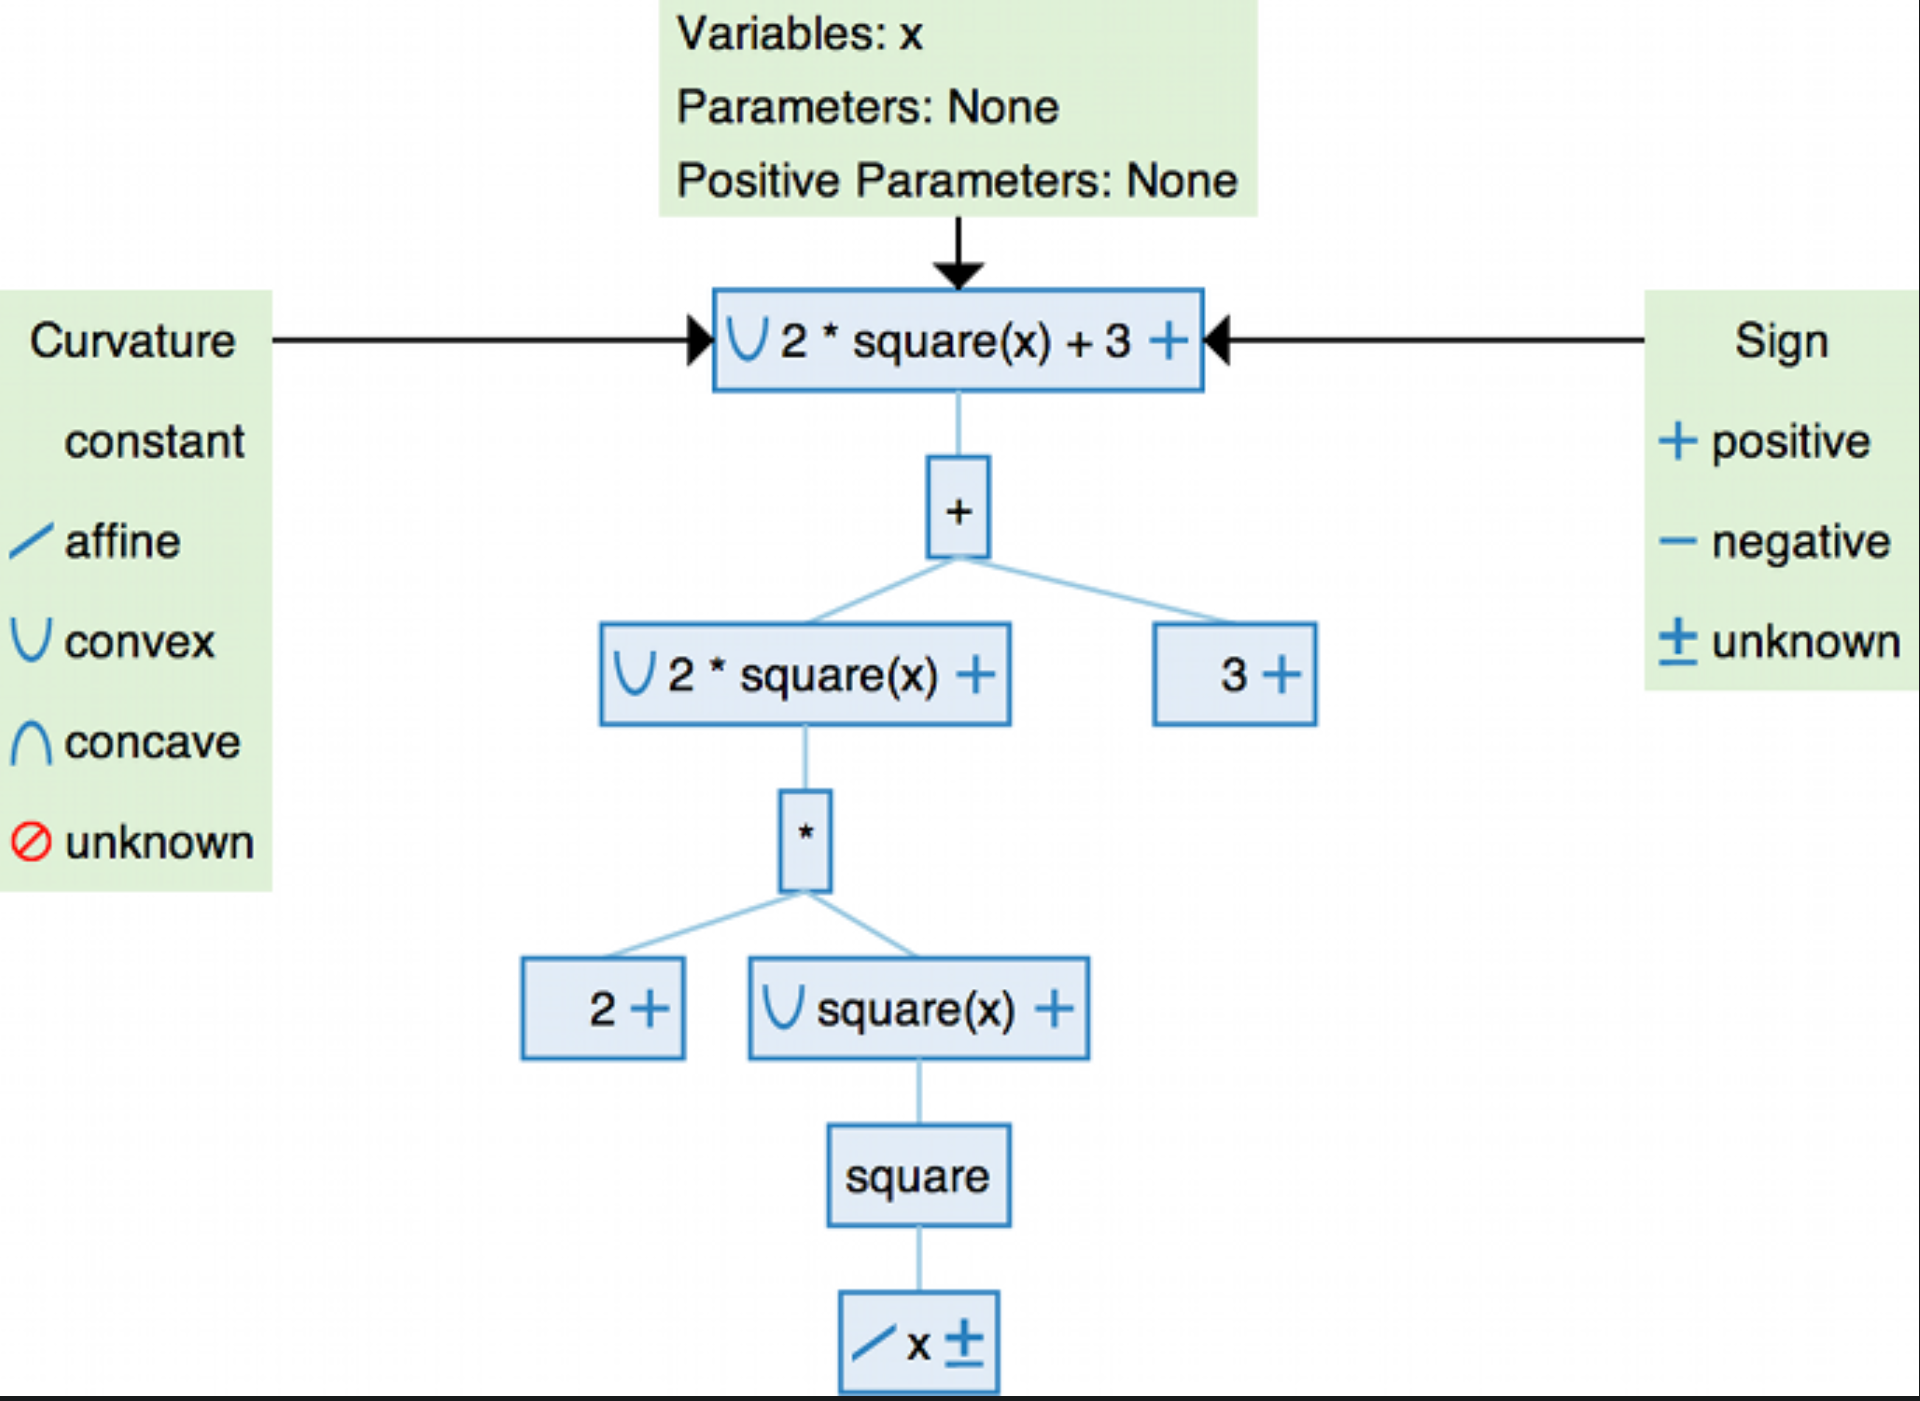
\includegraphics[scale=0.15]{figs/example3.png}
        \end{figure}
        \item \(f(x) = \mathtt{sqrt}(1 + x\textsuperscript{$\wedge$}2)\) \autocite{Rules}
        \begin{itemize}
            \item \(g(x) = x\textsuperscript{$\wedge$}2\) is a convex function (vide power function).
            \item \(g(x) + 1\) is a convex function (vide addition/subtraction by a constant).
            \item \(h(\cdot) = \mathtt{sqrt}(\cdot)\) is a concave function (vide power function) and nondecreasing. \(g\) should be convex to \(f = h \circ g\) be concave. But, since \(g\) is concave, this expression is not DCP-compliant.
        \end{itemize}
        \begin{figure}[H]
            \centering
            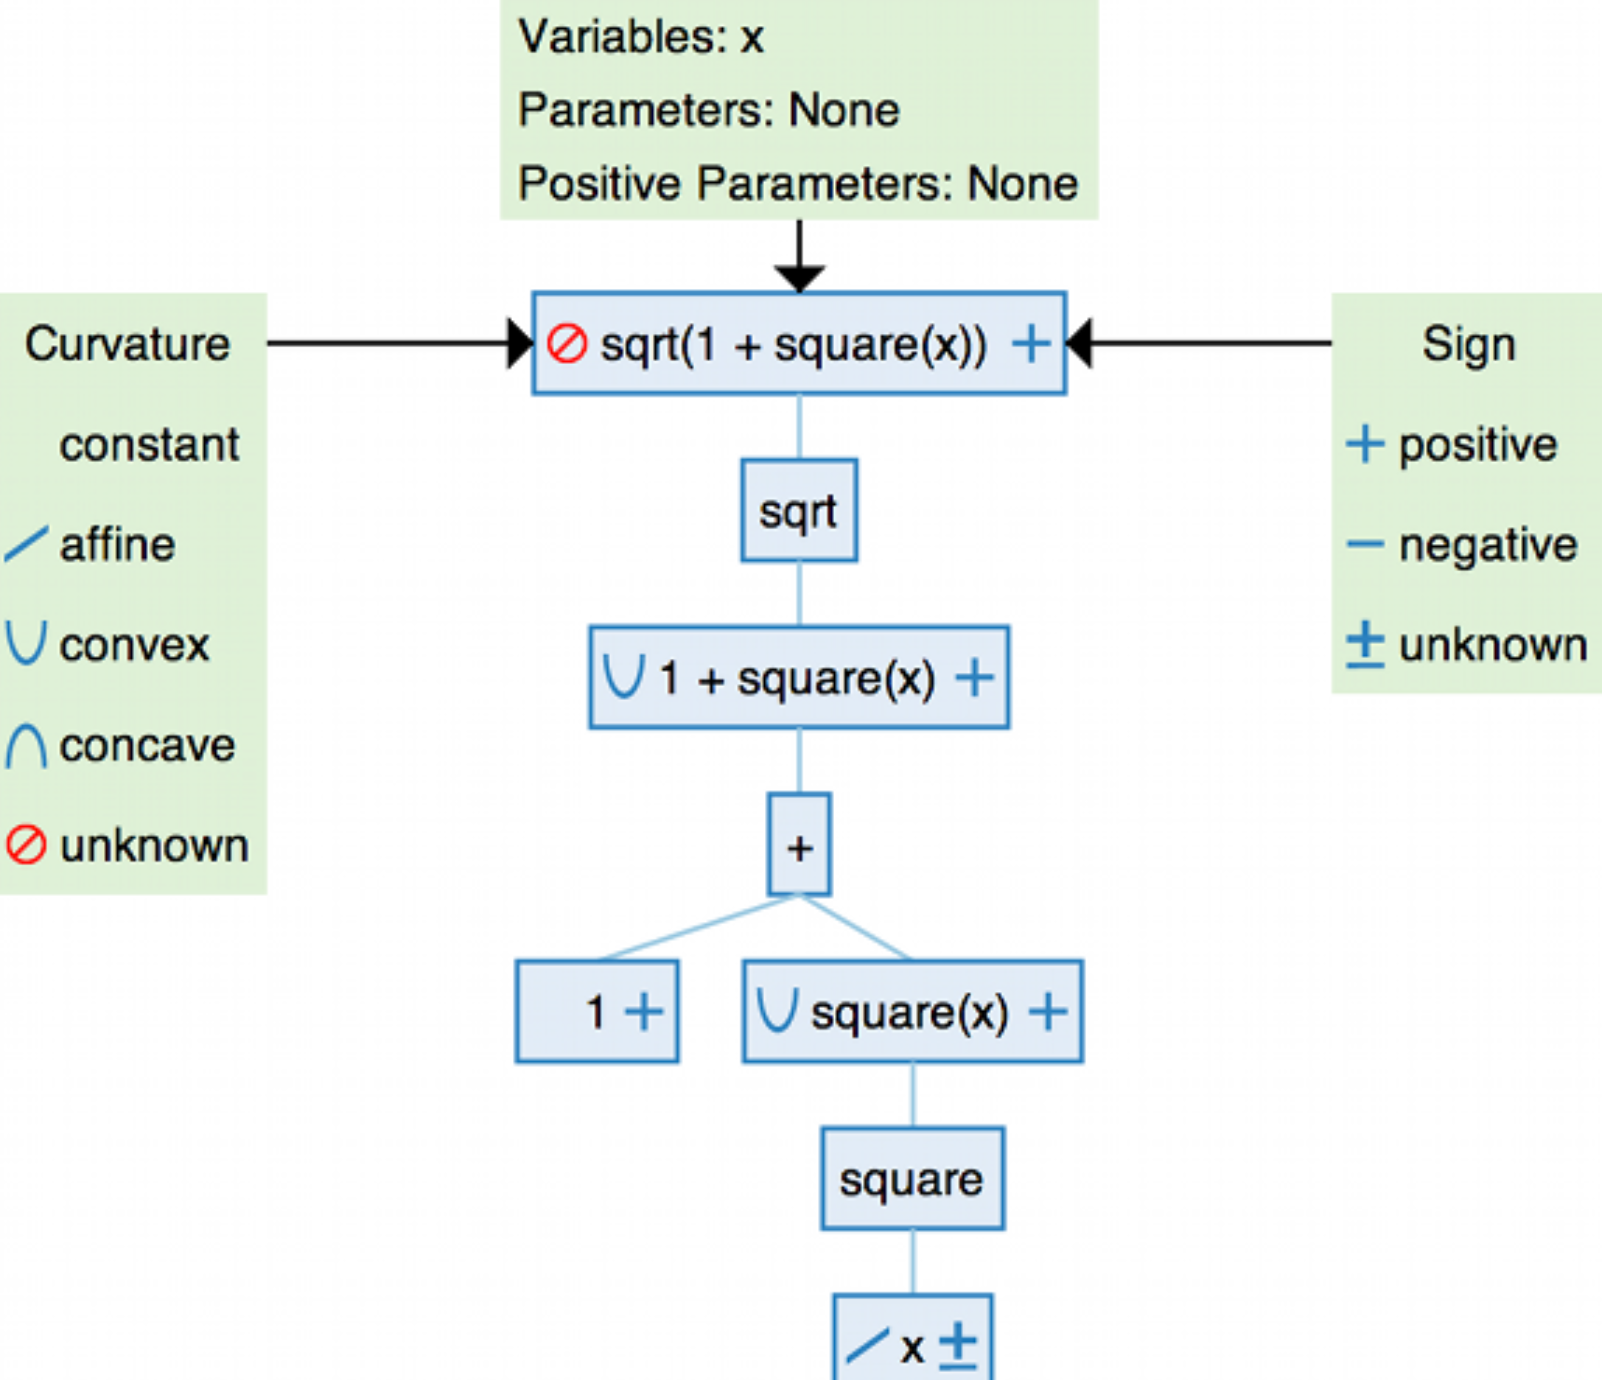
\includegraphics[scale=.15]{figs/example4.png}
        \end{figure}
    \end{itemize}

\subsection{DCP and constraints}
\begin{itemize}
	\item Type of constraints:
    \begin{itemize}
        \item Equality constraint.
        \item Inequality constraint (\(\leq\), \(\geq\), \(\preceq_K\), \(\succeq_K\)).
        \item Strict inequality constraint (\(<\), \(>\), \(\prec_K\), \(\succ_K\)).
    \end{itemize}
    \item Nonequalities is \emph{nerver} a constraint.
    \item For CVX packages, strict inequalities (\(<\), \(>\), \(\prec_K\), \(\succ_K\)) are analyzed as inequalities (\(\leq\), \(\geq\), \(\preceq_K\), \(\succeq_K\)). Thus, \emph{it is strongly recommended to only deal with nonstrict inequalities}.
    \item Convex and concave functions on CVX are interpreted as their \emph{extended-valued extensions} \autocite{DCPRulesetCVX}. This has the effect of automatically constraining the argument of a function to be in the function's domain.
    \begin{itemize}
        \item For example, if we form \texttt{sqrt(x+1)} in a CVX specification, \texttt{x} will automatically be constrained to be larger than or equal to \texttt{-1}.
        \item There is no need to add a separate constraint, \texttt{x>=-1}, to enforce this.
    \end{itemize}
\end{itemize}


\section{Methods of each optimization problem \autocite{macielSlidesOtimizacaoNaolinear}}
\begin{xltabular}[l]{\linewidth}{|>{\hsize=.25\hsize}X|>{\hsize=.25\hsize}X|}
    \hline
    Linear Optimization     & Simplex method     \\\hline
    Convex Optimization         & Branch-and-bound method        \\\hline
    Unconstrained Optimization         & subgradient, pattern search (also known as direct search, derivative-free search or black-box search)        \\\hline
    Constrained Optimization & Interior-points method\\\hline
\end{xltabular}

\printbibliography

\clearpage
\edef\hmm{\pdfpagewidth=\the\pdfpagewidth \pdfpageheight=\the\pdfpageheight\relax}
\pdfpagewidth=80cm
\pdfpageheight=60cm
\pagenumbering{gobble}
\newgeometry{top=1in,left=1in,textwidth=15in,textheight=9in}

\begin{figure}
    \centering
    \includestandalone{figs/optmization_types}
\end{figure}


% \restoregeometry
% \hmm
% Back to a standard page

% \begin{itemize}
%     \item All convex set is quasiconvex, but not all quasiconvex is convex.
%     \item It is possible to solve quasiconvex functions, even if it is not convex (see Algorithm 4.1). But not all quasiconvex functions that are nonconvex can be solved(?).
%     \item Superlevel set (a set) 3.3.6, all convex functions have all convex \(\alpha\) sub-level set, but not all functions that have convex \(\alpha\) sub-level set are convex (see slide 3.11).
% \end{itemize}

\end{document}